\PassOptionsToPackage{dvipsnames,svgnames,x11names}{xcolor}
\providecommand{\tightlist}{%
  \setlength{\itemsep}{0pt}\setlength{\parskip}{0pt}}
\documentclass[12pt]{article}
\usepackage[french]{babel}
\usepackage[utf8]{inputenc}
\usepackage{url}
\usepackage{array}
\usepackage{tabularx}
\usepackage{setspace}
\usepackage{abstract}
\usepackage{subfig}
\usepackage{listings}
\usepackage{amsmath}
\usepackage{graphicx}
\usepackage{iftex}
\usepackage{stmaryrd}
\usepackage[colorlinks]{hyperref}
\usepackage[top=2cm, bottom=2cm, left=2cm, right=2cm]{geometry}
\usepackage{titlesec}           % Pour changer la tailles ses sections/subsections...
\usepackage{algorithmic}        % Pour manipuler les algorithmes
\usepackage{algorithm}          % Pour manipuler les algorithmes
% \usepackage{algpseudocode}
\usepackage[absolute,overlay]{textpos} % Pour bouger les figures
\usepackage[nottoc]{tocbibind} %Includes "References" in the table of contents
\usepackage{listings}
\usepackage{xcolor}
\usepackage{fancyvrb}
\DefineVerbatimEnvironment{Highlighting}{Verbatim}{commandchars=\\\{\}}
\ifPDFTeX
  \usepackage[T1]{fontenc}
  \usepackage[utf8]{inputenc}
  \usepackage{textcomp} % provide euro and other symbols
\else % if luatex or xetex
  \usepackage{unicode-math} % this also loads fontspec
  \defaultfontfeatures{Scale=MatchLowercase}
  \defaultfontfeatures[\rmfamily]{Ligatures=TeX,Scale=1}
\fi
\usepackage{lmodern}
\ifPDFTeX\else
  % xetex/luatex font selection
  \setmainfont[]{Palatino}
  \setsansfont[]{Helvetica}
  \setmonofont[]{Menlo}
\fi
\allowdisplaybreaks
\colorlet{punct}{red!60!black}
\definecolor{background}{HTML}{EEEEEE}
\definecolor{delim}{RGB}{20,105,176}
\colorlet{numb}{magenta!60!black}
\lstdefinelanguage{minizinc}{
    morekeywords={
        constraint,int,
        maximize, solve, satisfy 
        var,
    },
    sensitive=true, % are the keywords case sensitive
    morecomment=[l][\em\color{ForestGreen}]{\%},
    %morecomment=[s]{/*}{*/},
    morestring=[b]",
}
\lstdefinelanguage{JavaScript}{
  keywords={typeof, new, true, false, catch, function, return, null, catch, switch, var, if, in, while, do, else, case, break},
  keywordstyle=\color{blue}\bfseries,
  ndkeywords={class, export, boolean, throw, implements, import, this},
  ndkeywordstyle=\color{darkgray}\bfseries,
  identifierstyle=\color{black},
  sensitive=false,
  comment=[l]{//},
  morecomment=[s]{/*}{*/},
  commentstyle=\color{purple}\ttfamily,
  stringstyle=\color{red}\ttfamily,
  morestring=[b]',
  morestring=[b]"
}

\lstset{
   language=JavaScript,
   backgroundcolor=\color{lightgray},
   extendedchars=true,
   basicstyle=\footnotesize\ttfamily,
   showstringspaces=false,
   showspaces=false,
   numbers=left,
   numberstyle=\footnotesize,
   numbersep=9pt,
   tabsize=2,
   breaklines=true,
   showtabs=false,
   captionpos=b
}
\lstset{
 basicstyle=\normalfont\ttfamily,
 language=caml,
 columns=[c]fixed,
 keywordstyle=\bfseries,
 upquote=true,
 commentstyle=,
 breaklines=true,
 frame=lines,
     numbers=left,
    numberstyle=\scriptsize,
    backgroundcolor=\color{background},
 showstringspaces=false,
 stringstyle=\color{blue},
 literate={'"'}{\textquotesingle "\textquotesingle}3
}
\lstdefinelanguage{json}{
    basicstyle=\normalfont\ttfamily,
    numbers=left,
    numberstyle=\scriptsize,
    stepnumber=1,
    numbersep=8pt,
    showstringspaces=false,
    breaklines=true,
    frame=lines,
    backgroundcolor=\color{background},
    literate=
     *{0}{{{\color{numb}0}}}{1}
      {1}{{{\color{numb}1}}}{1}
      {2}{{{\color{numb}2}}}{1}
      {3}{{{\color{numb}3}}}{1}
      {4}{{{\color{numb}4}}}{1}
      {5}{{{\color{numb}5}}}{1}
      {6}{{{\color{numb}6}}}{1}
      {7}{{{\color{numb}7}}}{1}
      {8}{{{\color{numb}8}}}{1}
      {9}{{{\color{numb}9}}}{1}
      {:}{{{\color{punct}{:}}}}{1}
      {,}{{{\color{punct}{,}}}}{1}
      {\{}{{{\color{delim}{\{}}}}{1}
      {\}}{{{\color{delim}{\}}}}}{1}
      {[}{{{\color{delim}{[}}}}{1}
      {]}{{{\color{delim}{]}}}}{1},
}
% Changement des commandes pour les algorithmes 
\renewcommand{\algorithmicrequire}{\textbf{Entrée(s)}}
\renewcommand{\algorithmicensure}{\textbf{Sortie(s)}}
\renewcommand{\algorithmicdo}{\textbf{faire}}
\renewcommand{\algorithmicforall}{\textbf{pour tout}}
\renewcommand{\algorithmicendfor}{\textbf{fin du pour}}
\renewcommand{\algorithmicif}{\textbf{si}}
\renewcommand{\algorithmicendif}{\textbf{fin du si}}
\renewcommand{\algorithmicthen}{\textbf{alors}}
\renewcommand{\algorithmicelse}{\textbf{sinon}}
\renewcommand{\algorithmicelsif}{\textbf{sinon si}}
\renewcommand{\algorithmiccomment}{\STATE //}
\setcounter{secnumdepth}{5}
\hypersetup{
    colorlinks,
    citecolor=black,
    filecolor=black,
    linkcolor=black,
    urlcolor=black
}

%pour ecrire chiffres romains
\makeatletter
\newcommand*{\rom}[1]{\expandafter\@slowromancap\romannumeral #1@}
\makeatother

\begin{document}

%régler l'espacement entre les lignes
\newcommand{\HRule}{\rule{\linewidth}{0.5mm}}


\titleformat{\chapter}{\bfseries\Large}{\arabic{chapter}.~}{0pt}{}   % Changer la taille des sections dans tout le document
\begin{titlepage}
      \center % Center everything on the page


      %----------------------------------------------------------------------------------------
      %	HEADING SECTIONS
      %----------------------------------------------------------------------------------------

      \textsc{\LARGE Sorbonne Université}\\[1.5cm] % Name of your university/college
      \textsc{\Large Rapport Final}\\[0.5cm] % Major heading such as course name
      {\large 19 Mai 2023}\\ % Date, change the \today to a set date if you want to be precise
      %\textsc{\large Minor Heading}\\[0.5cm] % Minor heading such as course title


      %----------------------------------------------------------------------------------------
      %	TITLE SECTION
      %----------------------------------------------------------------------------------------

      \vspace{2cm}
      \HRule \\[0.4cm]
      { \huge \bfseries Projet STL: \\ - \\ Interface pour Autobill}\\[0.7cm] % Title of your document
      \HRule \\[1cm]


      %----------------------------------------------------------------------------------------
      %	AUTHOR SECTION
      %----------------------------------------------------------------------------------------

      \begin{minipage}{0.4\textwidth}
            \begin{flushleft} \large
                  \emph{Auteurs:}\\
                  Brahima \textsc{Dibassi} \\
                  Zeid \textsc{Fazazi}\\
                  Yukai \textsc{Luo}
                  \vspace{2.5cm}
            \end{flushleft}
      \end{minipage}
      ~
      \begin{minipage}{0.55\textwidth}
            \begin{flushright} \large
                  \emph{Encadrants:} \\
                  Hector \textsc{Suzanne}\\ % Supervisor's Name
                  Emmanuel \textsc{Chailloux}\\ % Supervisor's Name
                  \textsc{}

                  \vspace{2.5cm}
            \end{flushright}
      \end{minipage}\\[1cm]

      % If you don't want a supervisor, uncomment the two lines below and remove the section above
      %\Large \emph{Author:}\\
      %John \textsc{Smith}\\[3cm] % Your name

      %----------------------------------------------------------------------------------------
      %	DATE SECTION
      %----------------------------------------------------------------------------------------


      %----------------------------------------------------------------------------------------
      %	LOGO SECTION
      %----------------------------------------------------------------------------------------

      
\includegraphics[scale=0.6]{Figures/Logo.png}\\[1cm] % Include a department/university logo - this will require the graphicx package

      %----------------------------------------------------------------------------------------

      \vfill % Fill the rest of the page with whitespace

\end{titlepage}
\newpage

{
      \hypersetup{linkcolor=}
      \setcounter{tocdepth}{3}
      \tableofcontents
}
\newpage

\section{Contexte du projet}\label{contexte-du-projet}
Dans le cadre de sa thèse sur l'analyse statique de consommation
mémoire d'un programme, notre tuteur de projet, Hector Suzanne, membre de l'équipe APR du laboratoire LIP6, a développé \cite{autobill}. \\
L'analyse statique est un ensemble de méthodes formelles permettant de
mesurer et détecter automatiquement des comportements ou des erreurs dans un
programme en examinant son code source. Parmi les usages les plus courants
de l'analyse statique, il y a le débogage pour identifier des erreurs
syntaxiques (fautes de frappe) ou l'usage de variables non déclarées ou
non-initialisées. D'autres outils emploient des heuristiques et des règles pour répondre à des problématiques d'optimisation de code ou de fiabilité/sécurité. Ces analyseurs statiques sont conçus dans le but d'améliorer la maintenabilité du code. \\
Autobill s'intéresse particulièrement à l'occupation mémoire d'un programme. Historiquement,
ce sujet de recherche a été plusieurs fois abordé dans divers travaux scientifiques, parmi eux, ceux de Jan Hoffmann et Steffen Jost sur l'analyse de consommation de ressources automatisé AARA
\cite{Hoffmann} (\emph{Automatic Amortized
      Resource Analysis}).\\
Cette technique suit un ensemble de règles d'inférences : chaque trait du langage analysé est annoté par ses bornes mémoire et on peut déduire la consommation mémoire que ce trait va engendrer. Pour déterminer ces bornes, l'AARA s'aide de l'analyse amortie par la méthode du potentiel. En effet, l'analyse amortie exploite la structure séquentielle des opérations sur des structures de données dynamiques pour calculer le coût total de cette séquence. Avec la méthode du potentiel, on attribue un potentiel aux structures de données manipulées, ce qui va affecter le coût que va avoir une opération sur cette structure. L’application de ces règles d'inférence sur l'ensemble des expressions du programme fournit une estimation correcte de ses bornes mémoires.
\begin{figure*}[!b]
      \centering
      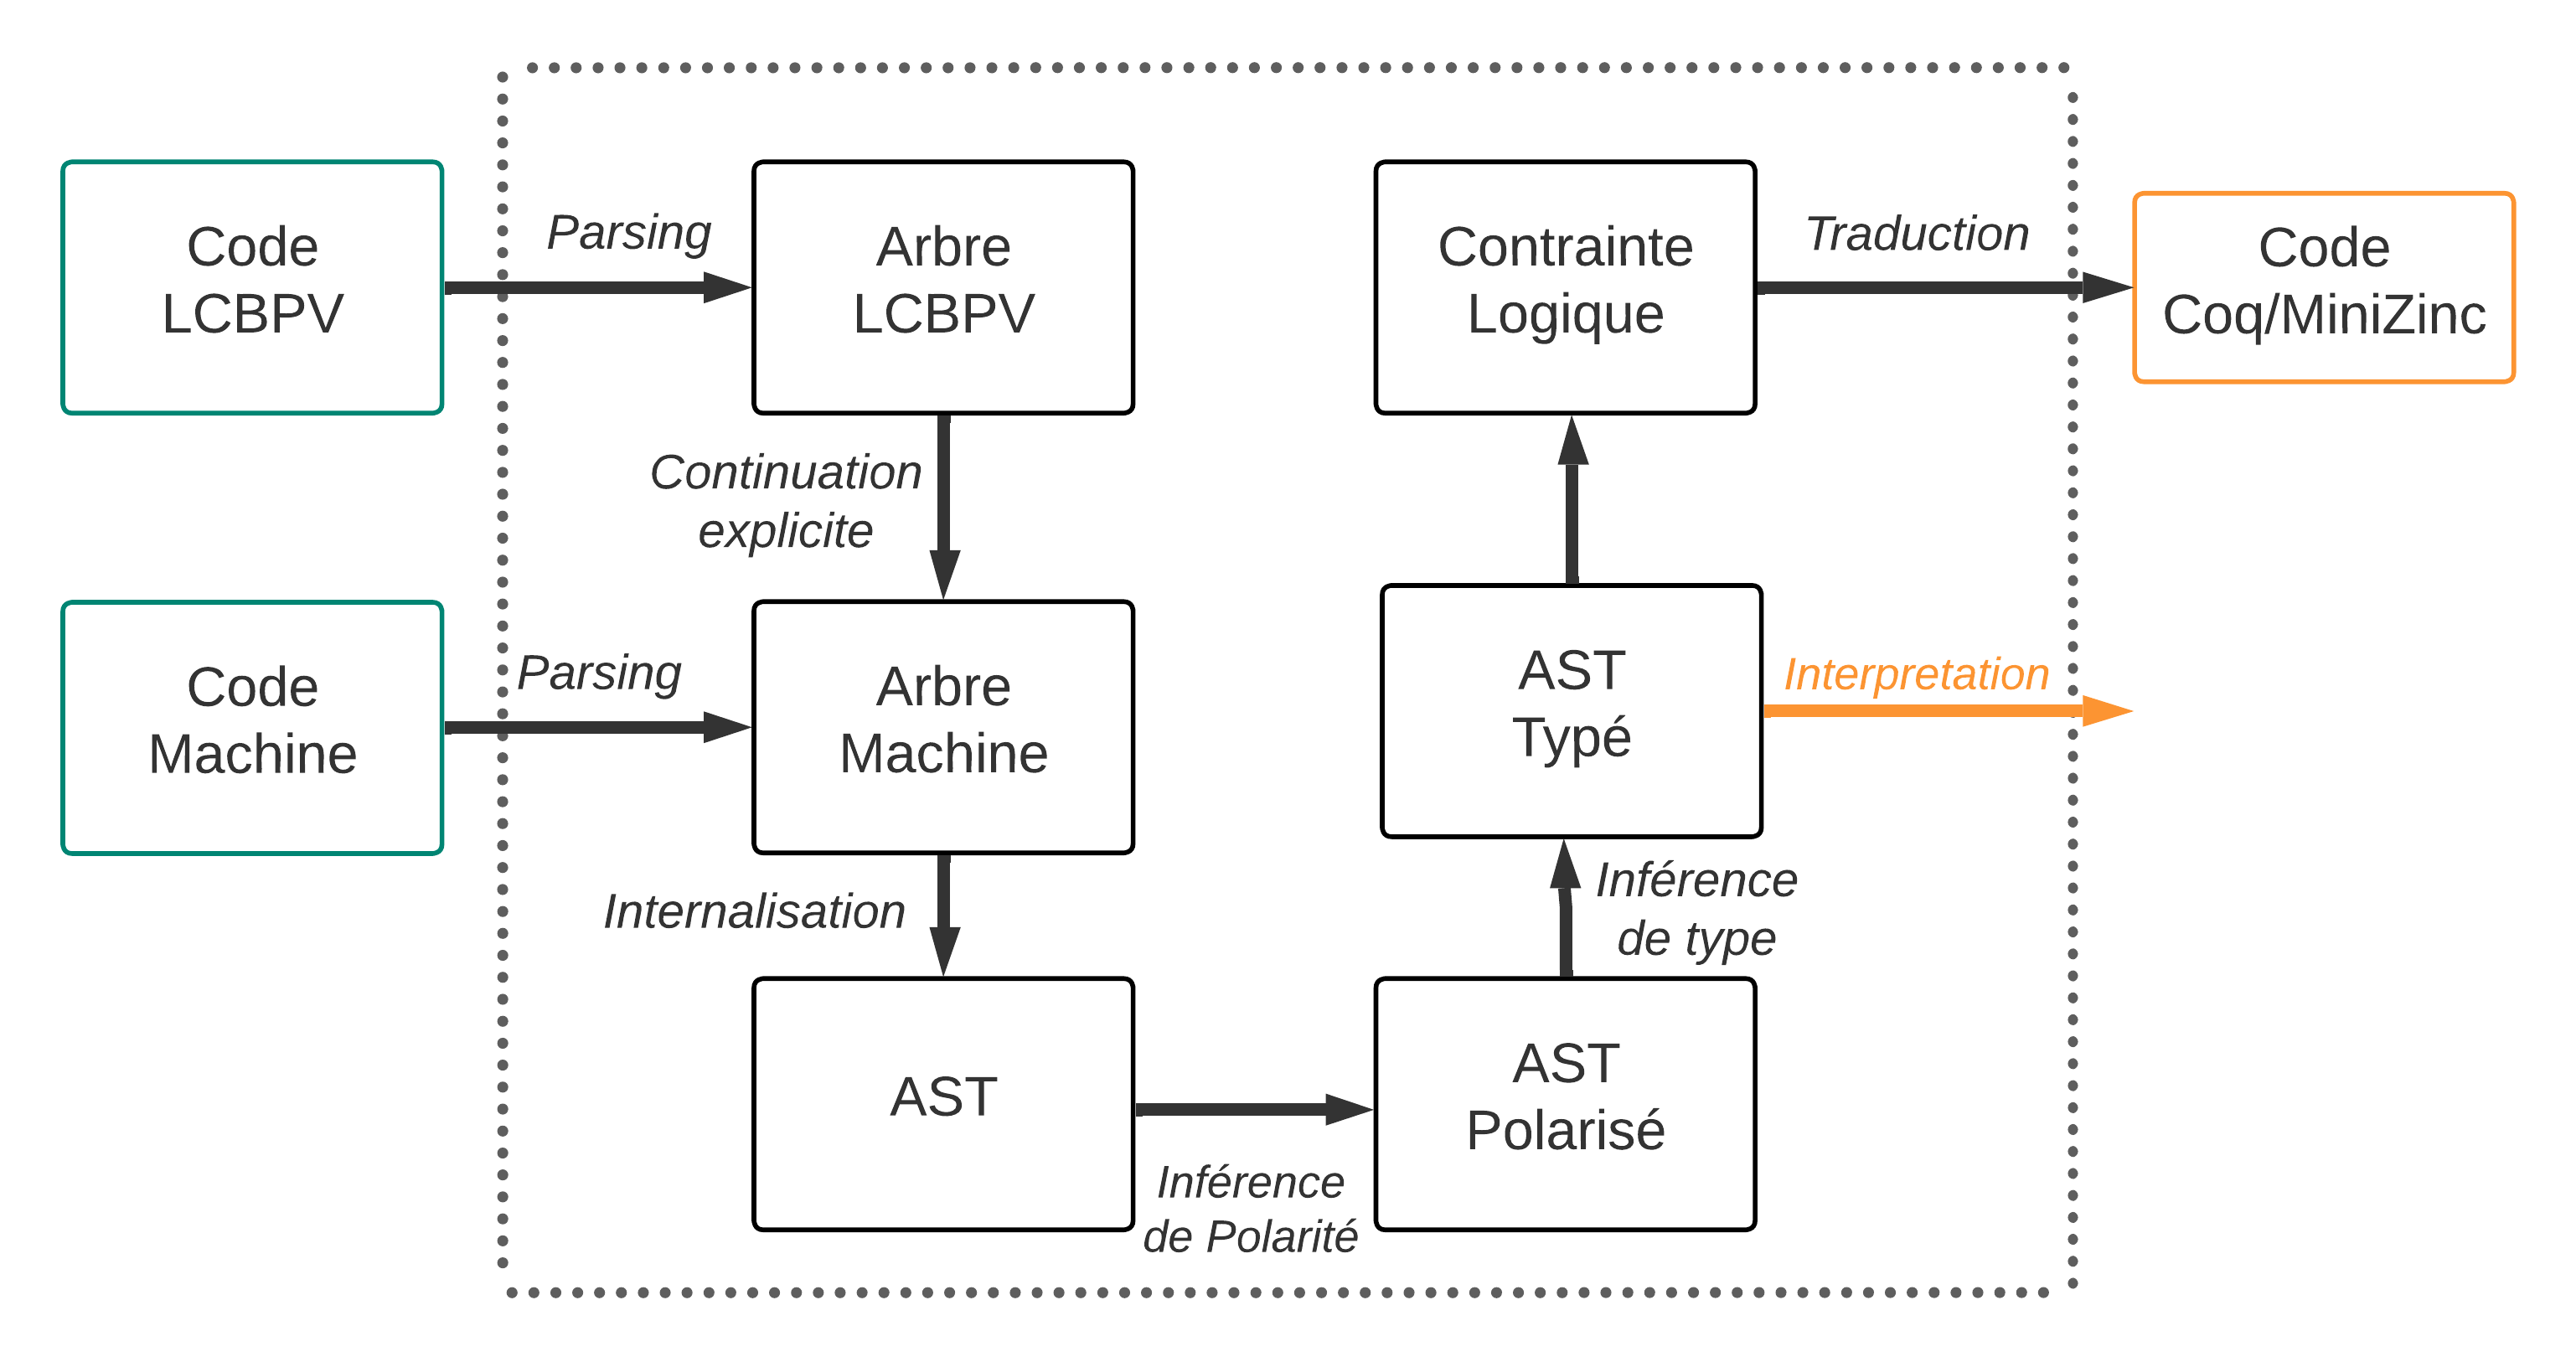
\includegraphics[scale=0.55]{Figures/Schema_Autobill.png}
      \caption{Représentation simplifiée d'Autobill\label{fig1}}
\end{figure*}

\pagebreak
\subsection{Historique et définitions}\label{historique-et-duxe9finitions}
Des langages de programmation expérimentaux ont vu le jour et ont implémenté cette analyse comme Resource Aware ML \cite{RAML}, un langage fonctionnel à la ML créé par Jan Hoffmann, Klaus Aehlig et Martin Hofmann.

\hypertarget{quest-ce-quautobill}{%
      \subsection{Qu'est-ce qu'Autobill ?}\label{quest-ce-quautobill}}

La proposition d'Hector Suzanne avec Autobill se différencie par un
niveau d'analyse plus précis sur les fermetures et les arguments
fonctionnels d'un programme par rapport à RAML. D'abord, parmi les entrées possibles
illustrées sur la gauche de la figure \ref{fig1}, Autobill ne supporte
uniquement que des programmes écrits soit en modèle machine propre à
Autobill, soit en \textbf{Call-By-Push-Value} (CBPV)
\cite{Levy}, avec ou sans continuation
explicite. \\

Call-By-Push-Value est un langage qui utilise un paradigme déjà éprouvé,
décrit dans la thèse de Paul Blain Lévy
\cite{Levy}. Dans CBPV, toutes les valeurs et fonctions sont stockées dans une pile. Lorsqu'une fonction est appelée, ses arguments sont placés sur la pile avant que la fonction elle-même ne soit ajoutée à la pile. Ce mécanisme permet de suivre de manière explicite les quantités de mémoire pour chaque valeur introduite/éliminée ou fonction appelée/terminée. Aussi,
le langage permet d'exprimer clairement les stratégies d'évaluation utilisées dans le code source : soit en \textbf{\textit{call-by-value}}, en évaluant les arguments avant de lancer l'opération, soit en \textbf{\textit{call-by-name}}, en évaluant les arguments uniquement lorsqu’ils seront effectivement utilisés dans la fonction appelée. Ainsi, on fixe quand les évaluations se déroulent, afin de mieux prédire la consommation de mémoire à chaque
étape du programme. Ces traits font de CBPV un langage de choix à analyser pour Autobill. \\

L'entrée est donc imposée. Ainsi, pour étendre l'usage d'Autobill à un
autre langage de programmation, un travail de traduction de ce langage
donné vers CBPV doit avoir lieu. Cela implique donc de comprendre le
langage que l'on compile, notamment les stratégies d'évaluations
implicites mises en œuvre, et de l'adapter aux caractéristiques uniques
de CBPV citées plus haut. \\

À partir d'une entrée en CBPV, Autobill traduit le programme en un code
machine avec continuations explicites, exprimant explicitement les
contraintes de taille qui s'appliquent sur l'entrée. Il l'internalise,
c'est à dire construit l'arbre syntaxique abstrait (AST) de ce
programme. Ensuite, Autobill infère dans l'AST le typage de ses
expressions ainsi que leurs polarités, pour démarquer les calculs et les
valeurs dans l'AST. Enfin, en sortie, on remarque dans la figure
\ref{fig1} la possibilité de tirer une interprétation du programme, mais
surtout de récupérer les contraintes dans un format MiniZinc
\cite{minizinc} ou Coq
\cite{coq}. Ce sont des outils des assistants
de preuve qui permettent, à l'aide d'un langage dédié, d'exprimer
explicitement des contraintes logiques. Autobill s'en sert pour décrire
les bornes mémoires nécessaires au fonctionnement d'un programme. On
peut alors traiter ces équations avec des solveurs, fournis aussi par
ces deux outils, pour prouver des propriétés de complexité temporelle ou
spatiale.

\newpage

\subsection{Objectifs du projet}\label{objectifs-du-projet}

Notre démarche se rapproche de celle de RAML
\cite{RAML} avec leur site officiel: offrir
une interface Homme-Machine accessible à tous et illustrant un sujet de
recherche en analyse statique.

Le sujet de notre projet STL va donc être de soutenir l'effort de
développement en proposant une interface sur le Web permettant la libre
manipulation de l'outil Autobill par des utilisateurs à travers un
environnement de développement sur navigateur. On souhaite
aussi faciliter l'utilisation de l'outil avec un langage fonctionnel pur
en entrée plus accessible, un \textbf{MiniML}. Cela nous contraint donc
à adapter cette nouvelle entrée pour qu'elle soit compatible avec
Autobill. Enfin, on se charge aussi de traiter les différentes sorties
standards et d'erreurs d'Autobill, notamment les expressions de
contraintes, afin de les passer à des solveurs externes, en tirer des
preuves de complexité et les afficher directement sur le client Web.

Par rapport à la chaîne d'instructions d'Autobill et à la Figure
\ref{fig1}, on se place donc en amont du code LCBPV en entrée et après
la sortie en code MiniZinc/Coq.

Notre charge de travail doit se diviser en plusieurs tâches principales:

\begin{itemize}
      \item
            L'implémentation du langage MiniML et sa traduction vers CBPV
      \item
            La mise en place d'une interface Web
      \item
            La mise en relation entre l'interface Web et la machine Autobill
      \item
            Le traitement des contraintes d'Autobill par un solveur externe
      \item
            Les tests de performances et comparaisons avec les solutions
            existantes
\end{itemize}

\begin{figure}
      \centering
      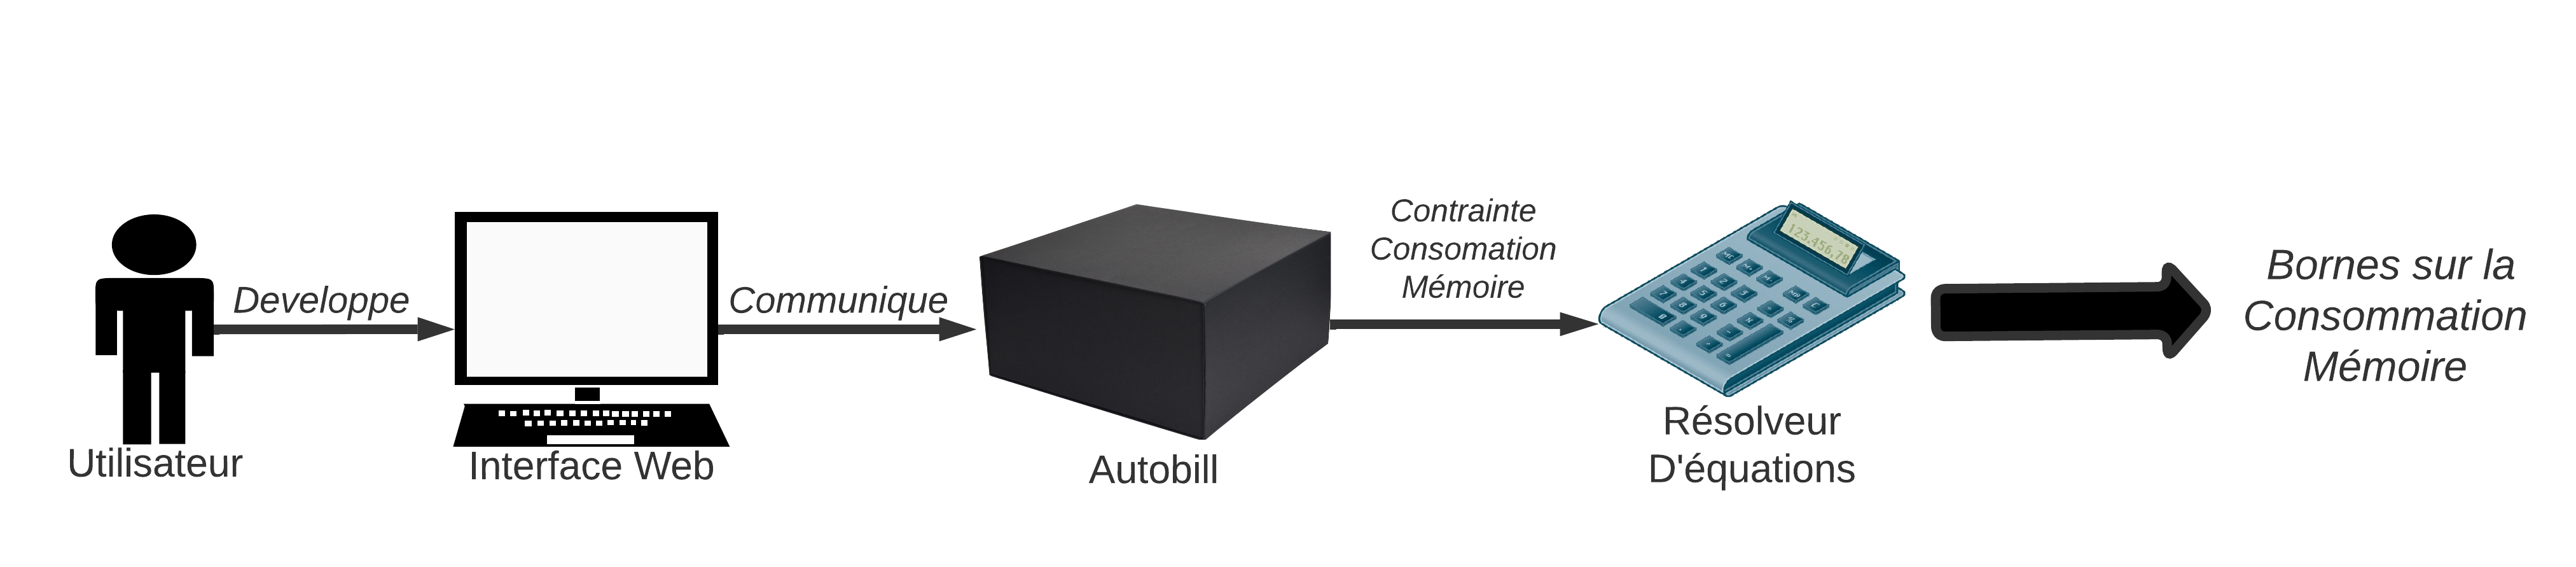
\includegraphics[scale=0.5]{Figures/DiagrammeHautNiveauPSTL.png}
      \caption{Représentation du système cible}
\end{figure}

\subsection{Processus de conception}\label{processus-de-conception}

Lors de la conception de l'interface, les contraintes étaient multiples.
La première était l'interopérabilité des technologies du projet. En
effet \textbf{Autobill} étant développé en \textbf{OCaml}, il était
nécessaire de trouver des moyens pour l'adapter à un environnement Web.
La seconde était qu'il fallait développer cette interface en simultané
avec \textbf{Autobill} et ajuster notre travail en fonction des besoins
courants de nos encadrants. Mais la plus importante d'entre elles était
le souhait de nos encadrants que l'application soit principalement côté
client afin de simplifier son déploiement.

Une fois ces contraintes établies, nous avons dû, tout au long de ce
projet, effectuer des choix, que ce soit en matière de design ou de
technologies. Nous tenons donc à travers ce rapport à mettre en lumière
ces décisions, tout en décrivant le travail qu'elles ont engendré.

\newpage

\hypertarget{interface-web}{%
      \section{Interface web}\label{interface-web}}

Dans l'optique de ne pas se restreindre dans l'utilisation d'outils
notamment au niveau du solveur de contraintes, le groupe s'est orienté
vers deux structures de projets différentes et indépendantes: l'une
fonctionnant avec un client unique, la seconde avec un serveur dédié et
un client qui expose ce serveur.

L'avantage réside dans le fait que, lors du développement, si un nouvel
outil est amené à être utilisé mais ne dispose de compatibilité sur
navigateur Web, alors le serveur peut répondre à ce problème. C'est
aussi un sujet de comparaison intéressant à présenter par la suite, que
ce soit au niveau des performances que du déploiement de ces solutions.

De cette démarche, il en résulte un code source d'environ 500 lignes,
client et serveur compris, faisant tourner notre IDE en ligne dans un
état fonctionnel.

\subsection{Client}

Une première approche tout client a été mise œuvre dès le début du
projet. Celle-ci permettait de garantir une facilité dans le déploiement
en ligne de notre solution. Cette partie se concentra sur la présentation de
notre client Web, de l'implémentation des fonctionnalités importantes et des problèmes rencontrés ainsi que leurs résolutions.

\subsubsection{Interopérabilité Web-Ocaml}\

Autobill est un projet entièrement codé en Ocaml, un langage de programmation multiparadigme compilé, et notre projet STL impose un environnement sur navigateur Web, fonctionnant exclusivement avec son langage de script Javascript. Avant de commencer tout codage, il est nécessaire de passer en revue l'état de l'art autour de la compilation et d'exécution de programmes Ocaml sur le Web. De ces recherches vont découler  des choix de conception qui vont nous impacter tout le long du semestre. \\

D'abord, il y'avait la piste des compilateurs vers WebAssembly. WebAssembly est un standard du W3C (World Wide Consortium) qui regroupe un bytecode (.wasm) et un environnement d'exécution compatible avec les navigateurs modernes Javascript. Le bytecode étant une représentation très bas niveau de l'exécutable, l'idée principale est de compiler un langage de programmation plus haut niveau, comme C/C++, Rust,.. vers bytecode. Ce bytecode est par la suite compilé par l'environnement d'exécution dans le langage machine de l'hôte. Tant que le support d'un langage de programmation est garanti par un compilateur WebAssembly, il est possible de programmer des applications web complètes dans le langage de son choix ou réinvestir des programmes codés dans ces langages dans une application codée avec des technologies Web. \\
Pour le cas d'Ocaml, cette possibilité est offerte grâce au post-processeur Wasicaml : il offre un binaire qui prend en entrée un bytecode Ocaml et un fichier .wasm de destination pour traduire chaque instruction dans son équivalent en WebAssembly. Ainsi, on pourrait générer nos fichiers .wasm à partir des binaires d'Autobill et de notre compilateur MiniML, les intégrer à notre applicatiton Web et les appeler avec Javascript en leur fournissant les options nécessaires. Cette solution demande néanmoins une dépendance à un projet encore en phase expérimentale, avec certains traits d'Ocaml non intégrés (notamment certaines fonctions du module Unix).\\
\begin{figure}
      \begin{lstlisting}
$ ocamlc -o hello hello.ml
$ wasicaml -o hello_wasm hello
\end{lstlisting}
      \caption{Chaine d'instructions pour générer le bytecode WebAssembly}
\end{figure}

La seconde piste émise par nos tuteurs de projet était l'utilisation de compilateurs Ocaml vers Javascript. La présentation du projet nous a notamment pointé vers Js\_of\_Ocaml. C'est une librairie contenant, entre autres, un compilateur qui transpile du bytecode OCaml en Javascript et propose une grande variété de primitives et de type pour manipuler des éléments Javascript depuis OCaml. L'API de Js\_of\_OCaml est suffisamment fournie pour développer entièrement des applications web complètes et fonctionnelles. On profite alors de l'expérience développeur offerte par Ocaml avec son style de programmation fonctionnelle en y intégrant les traits nécessaires pour construire des pages Web dynamiques.\\

Il est aussi possible de l'utiliser en coopération avec une base de code Javascript déjà rédigée grâce à la fonctionnalité d'export offerte par Js\_of\_Ocaml. En effet, on pourrait avoir dans un objet Javascript plusieurs méthodes correspondant chacune à un mode d'exécution différent d'Autobill. Chaque méthode prend en entrée le code MiniML à traiter et réalise les transformations nécessaires pour générer la sortie demandée. On peut aussi tirer profit des exceptions d'Ocaml et de la capture des sorties d'erreurs offerte par Js\_of\_Ocaml pour rediriger les messages d'erreurs et les afficher à l'utilisateur. Une fois l'objet exporté et le fichier Ocaml compilé vers Javascript, n'importe quel fichier Javascript du projet pourra ensuite importer l'objet et accéder aux méthodes définies précédemment. On garde ainsi une liberté sur le choix de technologies pour construire notre application.\\

\begin{figure*}[!b]
      \begin{lstlisting}[language=caml]
Js.export
    "ml"
    (object%js
       method translate code =
         let stderr_buff = Buffer.create 100 in
         Sys_js.set_channel_flusher stderr (Buffer.add_string stderr_buff);
         let lexbuf = Lexing.from_string ~with_positions:true (Js.to_string code) in
         let res = string_of_lcbpv_cst (translate_ML_to_LCBPV lexbuf)
         object%js
           val resultat = Js.string res
           val erreur = Js.string (Buffer.contents stderr_buff)
         end
    end)
\end{lstlisting}
      \caption{Création et exportation d'un objet Javascript avec une méthode de traduction de MiniML vers CBPV}
\end{figure*}
Enfin, une dernière piste suggérée a été l'utilisation de langages de programmation camélien compilables vers Javascript, comme ReasonML ou Rescript. En effet, ce sont tout deux des langages qui ont émergé d'Ocaml et permettent de créer dans un paradigme fonctionnel des applications web complexes. Ils profitent d'une syntaxe ML, d'outils et d'un support communautaire intéressant, faisant des deux langages des alternatives intéressantes pour le Web. Néanmoins, notre objectif principal est la manipulation de la librairie d'Autobill ainsi que celle de MiniML depuis le Web. La compatibilité avec les librairies en Ocaml n'est cependant pas garantie dans le contexte d'une compilation vers Javascript. \\

Notre groupe a donc opté pour un choix de conception assez flexible afin de nous adapter aux situations que l'on pourrait rencontrée dans le projet. Le client fonctionnera conjointement grâce à une partie Ocaml servie à l'aide de Js\_of\_Ocaml et une partie en Javascript, plus précisément en React.js, pour assurer les fonctionnalités propres à notre IDE.

\subsubsection{L'éditeur de code}\

L'idée initiale était de proposer une interface de développement intégrée sur le Web. Celle-ci devait proposer les outils nécessaires pour réaliser les trois tâches suivantes : analyser, écrire et déboguer du code. Pour répondre à ces besoins, plusieurs composants essentiels vont devoir fonctionner ensemble pour fournir l'expérience d'un IDE classique :
\begin{itemize}
      \item Un éditeur de code pratique et adapté à l'écriture de code dans notre langage MiniML.
      \item Un menu de navigation entre les programmes proposés par l'application ou créés par l'utilisateur
      \item Un menu de sélection entre différentes configurations d'analyses
      \item Une sortie standard et d'erreur pour afficher le retour de l'analyse d'Autobill \\
\end{itemize}

La question de l'éditeur de code s'est rapidement posée pour nous. En effet, c'est sur ce composant que va être concentrée l'expérience de l'application et nous avions la volonté de nous rapprocher au plus d'une prise en main similaire aux IDE modernes (Visual Studio Code, Eclipse, IntelliJ...). L'idée d'utiliser un simple champ de texte agrandi n'était donc pas envisageable. \\

En premier lieu, l'effort de développement a été mis dans la construction \textit{from Scratch} d'un éditeur de code. Cela a permis de fixer clairement les exigences et les fonctionnalités que nous attendions d'un éditeur de code moderne. Déjà, il devait proposer une expérience d'écriture correcte avec toutes les manipulations usuelles et attendues : le comptage des lignes, la recherche et le remplacement rapide d'une suite de caractères (Ctrl+F), le \textit{linting} d'erreurs... Enfin, il y'a le support du langage d'écriture des programmes. Par cela, il est question notamment de coloration syntaxique pour isoler les mots clés et symboles réservés du langage mais aussi de l'autocomplétion basique.  \\

\begin{figure}
      \centering
      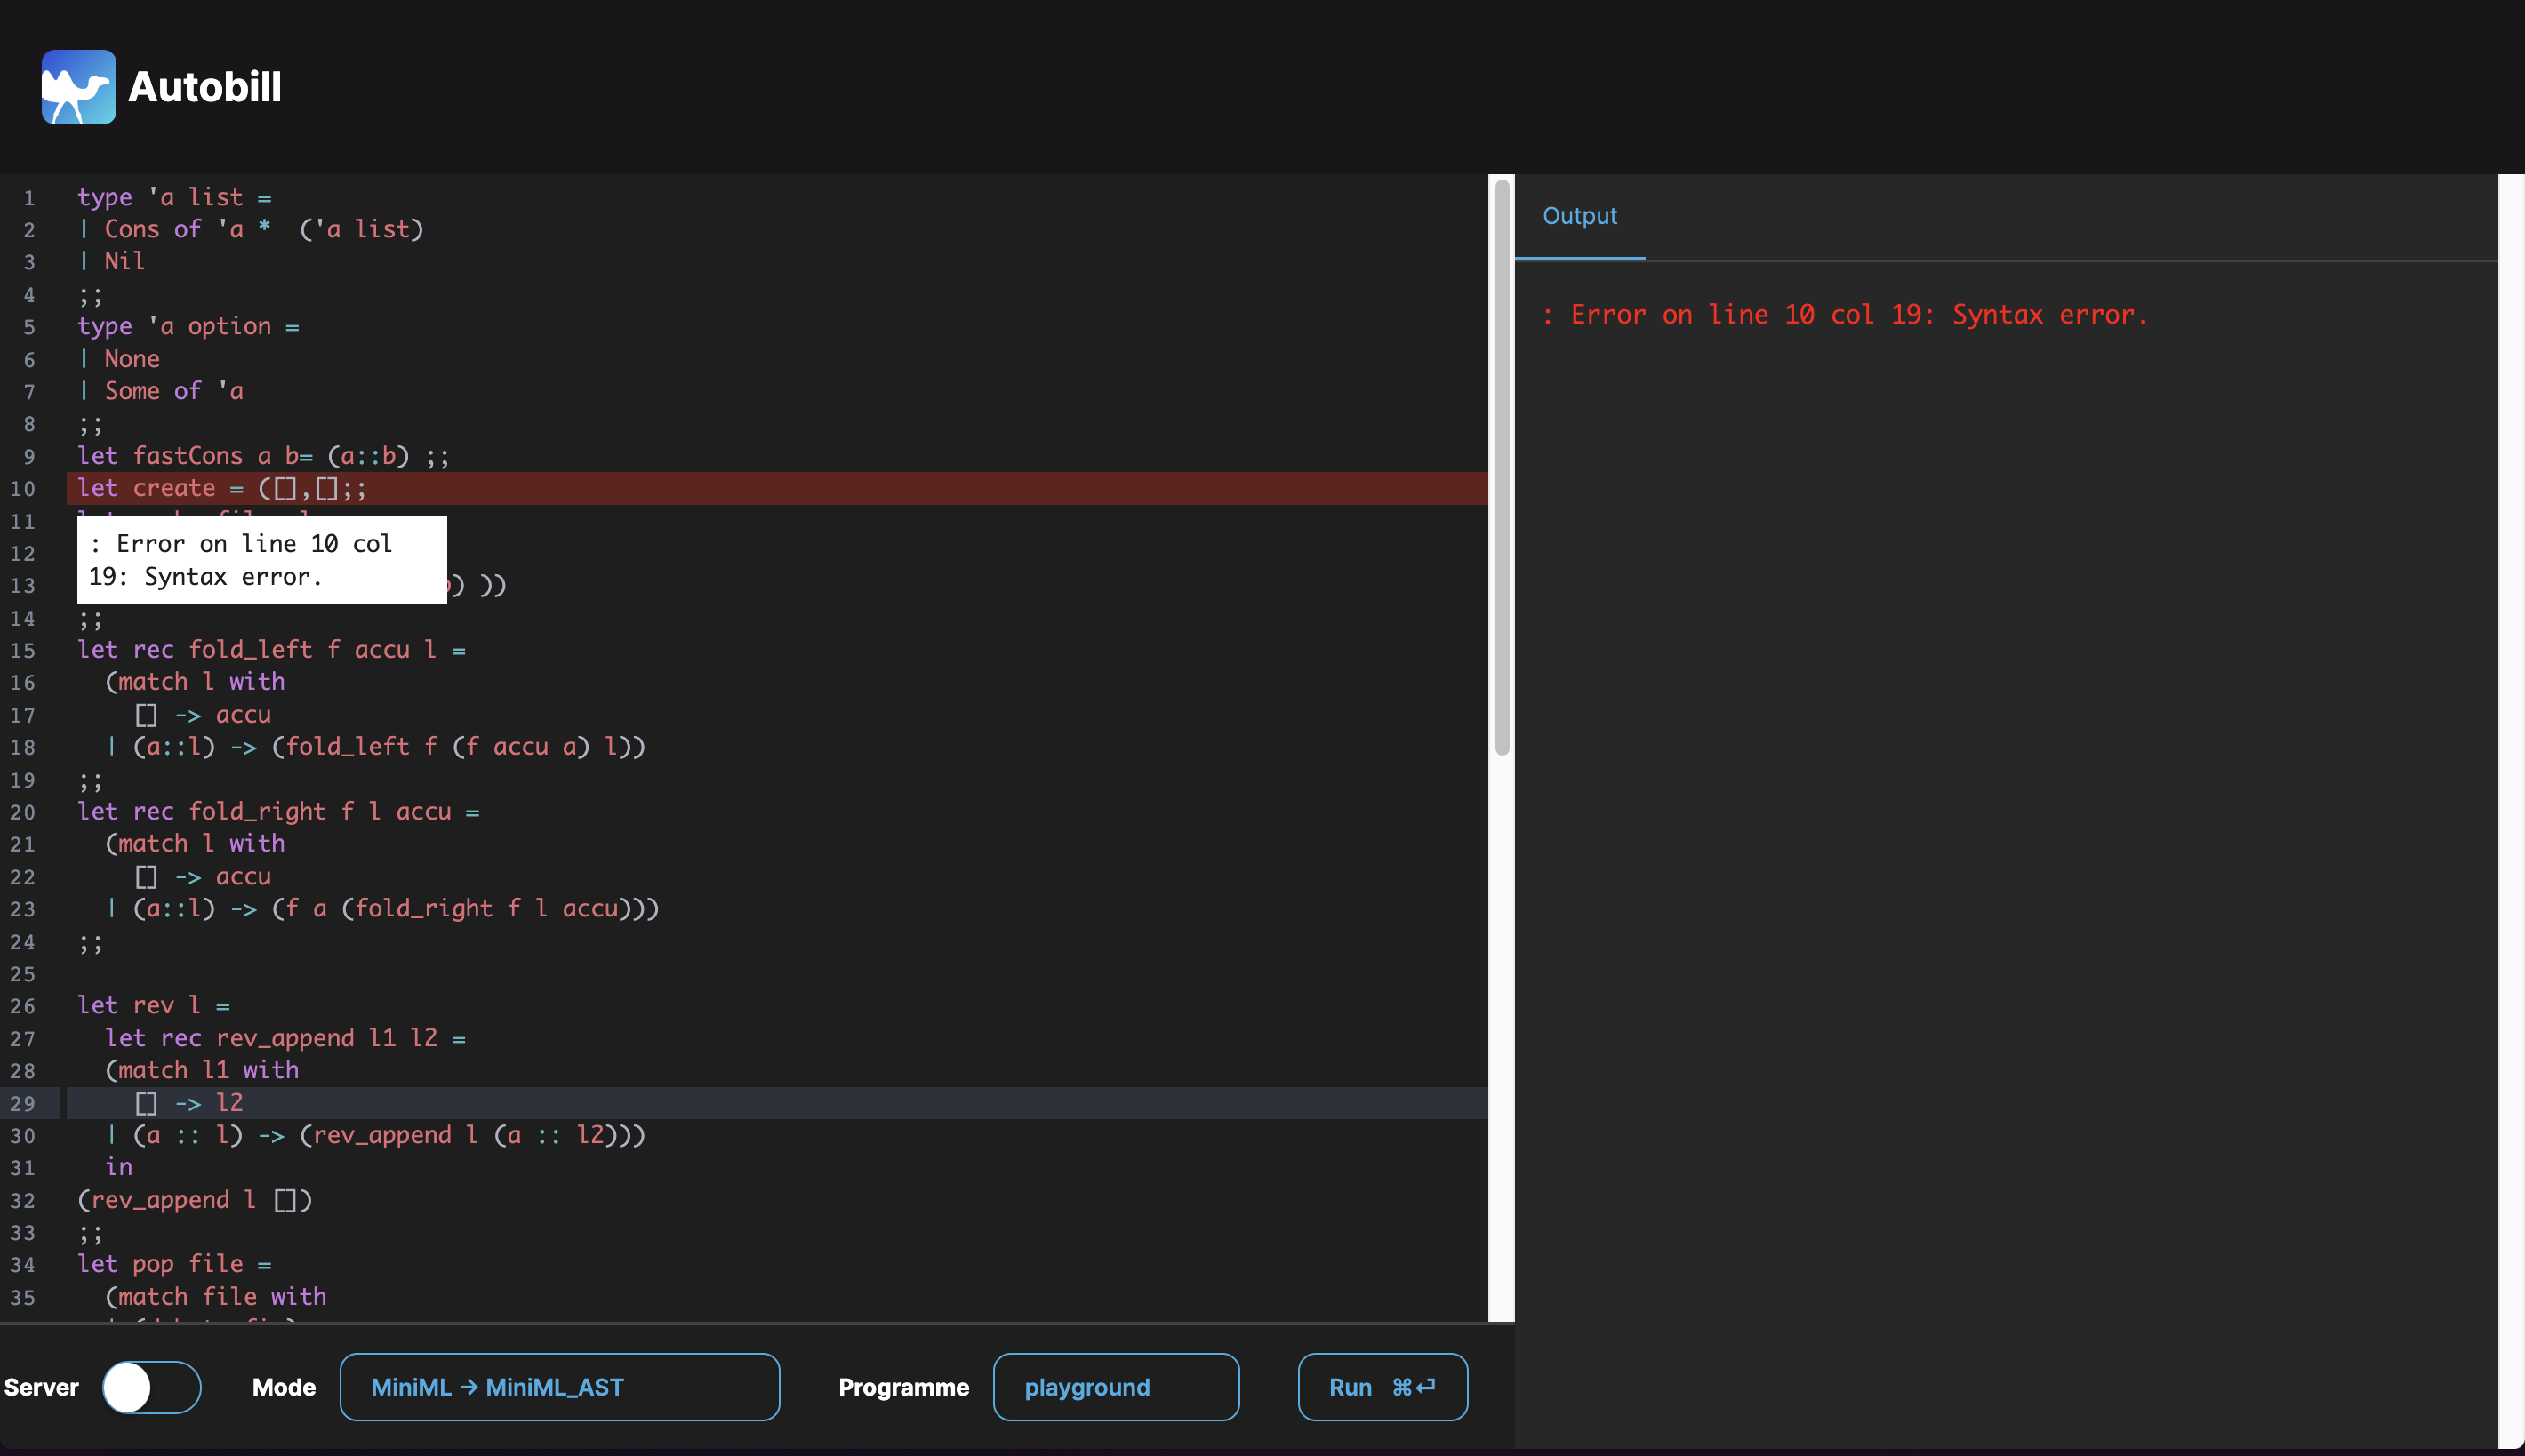
\includegraphics[scale=0.36]{Figures/screen.png}
      \caption{Interface pour Autobill, dans le scénario d'une erreur}
\end{figure}
L'examen de nos besoins nous a donc contraints à repousser l'idée d'une création d'un éditeur en partant de zéro. Délivrer les fonctionnalités citées plus haut tout en assurant la stabilité de la solution serait complexe et concentrerait beaucoup d'efforts sur ce composant, au détriment de chantiers clés comme le MiniML. C'est un élément de l'application d'autant plus important qu'il ne doit pas être négligé et demande à lui seul l'effort et le temps nécessaires à un projet universitaire. pour être réalisé. Nous nous sommes donc tournés vers des librairies et solutions déjà existantes afin de les intégrer dans notre projet. \\

Parmi les librairies disponibles, nous avons choisi CodeMirror. C'est un éditeur de code pour navigateur Web, disponible en libre de droits, qui peut s'intégrer à n'importe quelle application Web. Ses fonctionnalités sont exhaustives et il offre de multiples choix de personnalisations pour l'adapter à un langage spécifique. Nativement, il y'a le support intégré pour la syntaxe de langage à la ML comme Ocaml ou F\# : MiniML étant un substrat, on peut aisément créer notre fichier de configuration pour ne garder que les mots clés essentiels de notre langage et Codemirror s'occupe du parsing du code et de la coloration de chaque caractère. \\

Enfin, le \textit{linting} est disponible et permet de dynamiquement surligner des lignes de l'éditeur. Comme illustré dans la Figure 3, on peut, à la volée, afficher directement les parties du programme concernées par une erreur de l'analyse. En effet, quand une méthode de Js\_of\_Ocaml est appelée et qu'une exception est levée durant l'exécution, sa sortie d'erreur peut être redirigée et retournée directement au client. Côté Ocaml, on peut alors formater la sortie d'erreur avec les données de l'exception : la ligne de début et de fin, le type d'erreur rencontrée, la phase de l'analyse durant laquelle l'exception a été levée... \\
\begin{figure}
      \centering
      \begin{lstlisting}[language=json,firstnumber=1]
{
    "loc": {
        "beginning": { "line": 10, "column": 19},
        "end": {"line": 10, "column": 21}
    },
    "info": "Error on line 10 col 19: Syntax error."
}
\end{lstlisting}
      \caption{Sortie d'erreur Ocaml parsée}
\end{figure}

Côté Web, on peut parser la chaîne de caractères et récupérer le JSON parsé pour manipuler les informations sur l'erreur rencontrée (voir Figure 4). CodeMirror offre des fonctions permettant de manipuler l'état global de l'éditeur: son thème, son contenu, le langage de la coloration syntaxique, les options activées... On y retrouve surtout la liste des lignes qui composent l'éditeur. On peut alors leur affecter des changements de style pour les mettre en lumière ou faire apparaître une infobulle avec le message d'erreur si on passe la souris dessus... \\

On offre ainsi les outils nécessaires à l'utilisateur pour bien écrire et déboguer son code MiniML. Néanmoins, il faut encore compléter la \textit{pipeline} en traitant toutes les sorties possibles d'Autobill, notamment les équations sur les contraintes mémoires du programme analysée qu'il va falloir résoudre.

\subsubsection{La résolution de contraintes}\

Autobill exprime les contraintes mémoires qui s'appliquent à un programme dans des formats proches d'équations mathématiques. Il propose de type de sortie : une sous Coq et une sous MiniZinc. Nous nous concentrerons principalement sur MiniZinc dans cette partie, Coq n'étant pas encore totalement opérationnel et demandant des ressources qui dépassent le cadre du Master d'informatique. \\

MiniZinc est un langage permettant de décrire des problèmes de manière déclarative à l'aide de contraintes logiques. Il fournit des éléments de syntaxe et de notations très similaires à la programmation et aux mathématiques pour rédiger des modèles qui, lorsqu'ils seront passés à des compilateurs et des solveurs dédiés, vont répondre à des problématiques d'optimisation ou de satisfiabilité. Dans notre cas, on s'intéresse à l'optimisation : on veut déterminer les bornes mémoires minimum du programme passée à Autobill.
Néanmoins, on rencontre un problème similaire qu'avec Autobill : la librairie est codée en C++, langage compilé, incompatible avec l'environnement Web. Là encore, l'option de WebAssembly est envisageable avec un compilateur comme Emscripten qui supporte la traduction de code C/C++ vers bytecode WebAssembly. Ici, la librairie core de MiniZinc est beaucoup plus fournie et ne contient pas un point d'entrée direct explicite, comme avec le binaire d'Autobill. La compilation devient alors une tâche plus compliquée et la manipulation sûre de l'outil n'est pas non plus garantie par la suite.
\begin{figure*}[!b]
      \centering
      \begin{lstlisting}[language=minizinc]
        int: n;
        var 1..n: x; var 1..n: y;
        constraint x+y > n;
        solve satisfy;
    \end{lstlisting}
      \caption{Exemple de modèle en MiniZinc}
      \label{Simple modèle pour déterminer la satisfiabilité d'une équation}
\end{figure*} \newpage
\begin{lstlisting}[language=javascript]
    const model = new Model()
    model.addFile("playground.mzn", code)
    const solve = await model.solve({
      options: {
        solver: "gecode",
      },
    })
\end{lstlisting}
\iffalse
      \begin{itemize}
            \item
                  \textbf{HTML / CSS / Javascript (JS)}: Il s'agit de la suite de
                  langages principaux permettant de bâtir l'interface Web souhaitée. On
                  a ainsi la main sur la structure de la page à l'aide des balises HTML,
                  du style souhaité pour l'éditeur de code avec le CSS et on vient
                  apporter l'interactivité et les fonctionnalités en les programmant
                  avec Javascript, complété par la librairie React.
            \item
                  \textbf{React.js} \cite{react}: React.js est
                  une bibliothèque JavaScript \emph{open-source} pour la création
                  d'interfaces utilisateur,utilisée pour la création d'applications web
                  modernes et interactives. Parmi les avantages de cette technologie, il
                  y a l'utilisation du Virtual DOM (Document Object Model) qui permet
                  une mise à jour plus efficace et rapide des éléments d'une page. Le
                  Virtual DOM est une représentation virtuelle d'un arbre DOM qui est
                  stockée en mémoire et mise à jour en temps réel en fonction des
                  interactions de l'utilisateur avec l'interface. On modifie seulement
                  les éléments impactés, et non l'ensemble du DOM de la page, ce qui se
                  traduit par des temps de réponse plus rapides et des meilleures
                  performances.\newline  Aussi, React est basé sur la programmation
                  orientée composant. L'interface utilisateur est décomposée en petits
                  composants réutilisables, chacun étant responsable de l'affichage
                  d'une partie spécifique de l'interface. Chaque composant est construit
                  de manière indépendante et peut être utilisé à plusieurs endroits dans
                  une application. Cette approche modulaire rend l'interface plus
                  flexible et maintenable. D'autres solutions concurrentes et valables
                  telles que Angular.js \cite{angularjs} ou
                  Vue.js \cite{vuejs} proposent une expérience
                  développeur similaire.\newline  Néanmoins, ces dernières sont bien
                  moins recherchées sur le marché du travail que React. Nous voulions à
                  travers ce projet nous former et pratiquer une technologie très en
                  vogue et que l'on pourra facilement réinvestir plus tard dans notre
                  parcours professionnel.
            \item
                  \textbf{CodeMirror} \cite{codemirror}:
                  C'est une librairie Javascript permettant d'intégrer un éditeur de
                  code puissant, incluant le support de la coloration syntaxique, de
                  l'autocomplétion ou encore le surlignage d'erreurs. Les
                  fonctionnalités de l'éditeur sont grandement extensives et permettant
                  même la compatibilité avec un langage de programmation personnalisé
                  comme MiniML. Enfin, CodeMirror est disponible sous licence MIT, libre
                  de droits.
            \item
                  \textbf{OCaml} \cite{Minsky_Ocaml}
                  \cite{chailloux}
                  \cite{Leroy} + \textbf{Js\_of\_OCaml}
                  \cite{js_of_ocaml}: Afin de manipuler la
                  librairie d'Autobill, il est nécessaire de passer par OCaml pour
                  traiter le code en entrée et en sortir des équations à résoudre ou des
                  résultats d'interprétations. Pour faire le pont entre Javascript et
                  OCaml, on utilise Js\_of\_OCaml, une librairie contenant, entre
                  autres, un compilateur qui transpile du bytecode OCaml en Javascript
                  et propose une grande variété de primitive et de type pour manipuler
                  des éléments Javascript depuis OCaml. L'API de Js\_of\_OCaml est
                  suffisamment fournie pour développer entièrement des applications web
                  complètes et fonctionnelles.\newline  Pour ce projet, il sert surtout
                  pour interagir avec Autobill et la librairie de MiniML depuis le
                  client Web. Dans un fichier \texttt{main.ml}, on exporte un objet
                  Javascript contenant plusieurs méthodes correspondant chacune à un
                  mode d'exécution différent d'Autobill. Chaque méthode prend en entrée
                  le code MiniML à traiter et réalise les transformations nécessaires
                  pour générer la sortie demandée.\newline  Néanmoins, en l'absence de
                  sortie standard ou d'erreurs, les messages d'exceptions d'Ocaml, par
                  exemple, n'apparaissent que dans la console Javascript du navigateur.
                  Js\_of\_ocaml met à notre disposition un module \texttt{Sys\_js} qui
                  offre des primitives permettant de capturer les possibles messages sur
                  les sorties et les rediriger dans des buffers. Ces buffers peuvent
                  être convertis en chaînes de caractères et retournés au client par la
                  suite.\newline  La question s'est posée de l'intérêt de Js\_of\_OCaml
                  comparé à d'autres technologies comme ReasonML
                  \cite{reasonml} ou Rescript
                  \cite{rescript}. En effet, ce sont tout
                  deux des langages qui ont émergé d'Ocaml et permettent de créer dans
                  un paradigme fonctionnel des applications web complexes. Des
                  compilateurs pour transpiler du code Rescript (Bucklescript) ou
                  ReasonML vers Javascript existent et ReasonML permet même de compiler
                  vers du code en React.\newline  Néanmoins, notre objectif principal
                  est la manipulation de la librairie d'Autobill ainsi que celle de
                  MiniML depuis le Web. Ces deux technologies affichent des syntaxes
                  différentes de celle d'OCaml, ce qui empêche toute compatibilité avec
                  les bibliothèques d'OCaml. Js\_of\_OCaml en complément avec un client
                  en React correspond donc à un bon compromis dans notre cas d'étude.
      \end{itemize}
      \begin{itemize}
            \item
                  \textbf{MiniZinc} \cite{minizinc} : À la
                  génération des expressions de contraintes, Autobill retourne une
                  sortie au format MiniZinc. Ce langage permet de décrire des problèmes
                  de manière déclarative à l'aide de contraintes logiques. L'objectif
                  avec MiniZinc est de calculer les bornes mémoires minimums pour
                  satisfaire les contraintes mémoires du programme et d'afficher, sous
                  forme d'équation, le résultat dans la sortie de notre IDE. Son API
                  prend en charge une large gamme de solveurs. Aussi, il dispose d'une
                  grande communauté d'utilisateurs et de contributeurs, ce qui nous
                  permet de trouver nombreuses ressources disponibles pour
                  l'apprentissage et le dépannage.\newline  Sa librairie est codée en
                  C++ mais il reste utilisable dans notre interface Web grâce à Web
                  Assembly. C'est un format binaire de code exécutable qui permet de
                  porter des applications codées dans des langages de programmation sur
                  le Web. Grâce à des compilateurs vers Web Assembly, comme Emscripten
                  pour C/C++, on peut lancer des tâches intensives de résolution de
                  contraintes, depuis n'importe quel navigateur Web moderne.
      \end{itemize}
\fi
\pagebreak

\hypertarget{serveur-client}{%
      \subsection{Serveur + client}\label{serveur-client}}

Dans le stade actuel d'Autobill, une architecture avec un client seul
peut répondre aux exigences du projet STL. Néanmoins, au fur et à mesure que le projet avançait, nous nous sommes rendu compte d'un problème. Autobill évolue constamment et rien ne garantit que ses itérations suivantes puissent
être supportées par notre solution. Par exemple, la utilisation de la librairie core de Mini-Zinc peut échouer en mode client unique. Dans l'optique de rendre notre solution plus flexible et \emph{futureproof}, une nouvelle version de notre interface, qui déporte les tâches complexes vers un serveur
distant, a été développée.

On a souhaité aussi adapter le client pour qu'il opère dans ces deux
architectures différentes. Ainsi, dans notre environnement de
développement, on peut facilement faire la bascule entre un mode de
fonctionnement local/synchrone et un mode distant/asynchrone.

\hypertarget{schuxe9ma-de-communication}{%
      \subsubsection{Schema de Communication}\label{schuxe9ma-de-communication}}

\begin{figure}[!b]
      \centering
      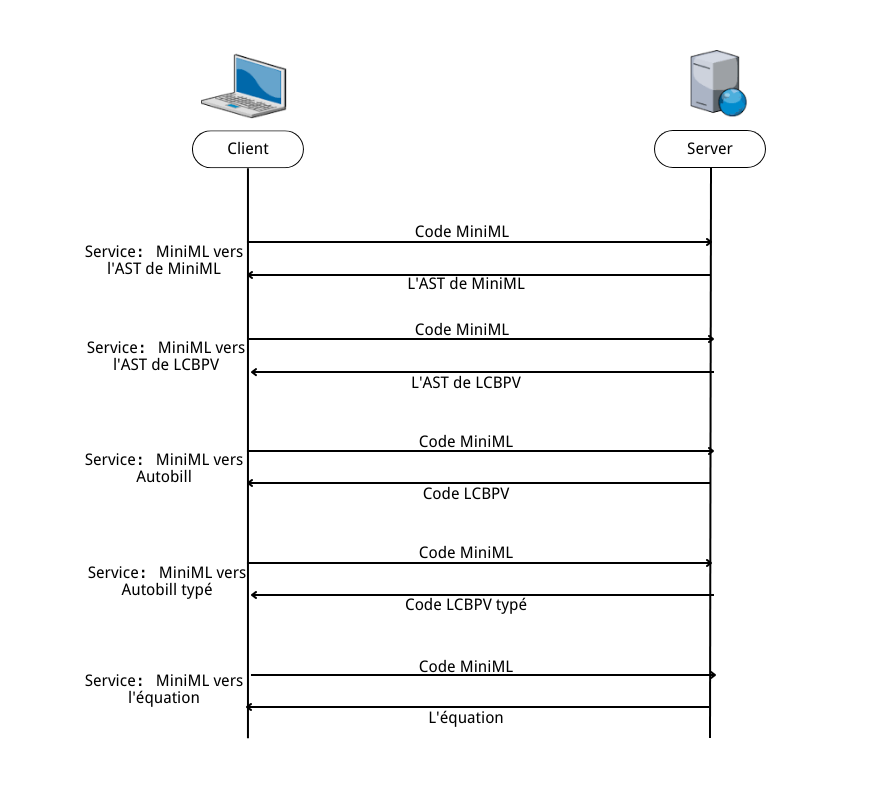
\includegraphics[scale=0.5]{Figures/CommunicationMiniML.png}
      \caption{Schéma de communication}
\end{figure}


Nous vouslons diviser notre architecture Client-Server en deux partie, la partie MiniML et la partie résolution de contraintes. \\
Dans la partie MiniML, nous avons mis en place 5 services principaux en utilisant le protocole HTTP (voir Figure 8): \emph{'/MiniML/toMiniMLAST'}, \emph{'/MiniML/toLCBPV'}, \emph{'/MiniML/toAutobill'}, \emph{'/MiniML/toAutobillType'} et \emph{'/MiniML/toEquation'}. \\
Pour le service \emph{'/MiniML/toMiniMLAST'}, le client envoit le code du MiniML au server via une rêquete POST. Le server le transforme vers l'AST de MiniML et le renvoit au client.\\
Pour le service \emph{'/MiniML/toLCBPV'},le client envoit le code du MiniML au server via une rêquete POST. Le server le transforme vers l'AST de LCBPV et le renvoit au client.\\
Pour le service \emph{'/MiniML/toAutobill'}, le client envoit le code du MiniML au server via une rêquete POST. Le server le transforme vers le code d'Autobill et le renvoit au client.\\
Pour le service \emph{'/MiniML/toAutobillType'}, le client envoit le code du MiniML au server via une rêquete POST. Le server le transforme vers le code d'Autobill typé et le renvoit au client.\\
Pour le service \emph{'/MiniML/toAutobillType'}, le client envoit le code du MiniML au server via une rêquete POST. Le server le transforme vers l'équation résultant de l'analyse statique et le renvoit au client.\\


\subsubsection{La résolution de contraintes}\

Dans la partie résolution de contraintes, nous avons un service \emph{'/minizinc/gecode'} qui éxecute le code MiniZinc. Le client envoie le code de MiniZinc au serveur via une requête POST. Le serveur écrit le code dans un fichier temporaire puis l'exécuter à l'aide de l'exécutable de ligne de commande minizinc avec le solveur Gecode (voir Figure.9), et renvoie le résultat au client.

\begin{figure}[!b]
      \centering
      \begin{lstlisting}[language=javascript]
    const fs = require('fs');
    const tmpFile = './temp.mzn';
    fs.writeFileSync(tmpFile, code);
    const cmd = `minizinc --solver Gecode ${tmpFile}`;
    exec(cmd, (error, stdout, stderr) => {
        fs.unlink('temp.mzn', (err) => {
            if (err) throw err;
        });
    }
\end{lstlisting}
      \caption{Exécution de code Minizinc}
\end{figure}

\hypertarget{schuxe9ma-de-communication}{%
      \subsubsection{Schema de Communication}\label{schuxe9ma-de-communication}}

\begin{figure}[!b]
      \centering
      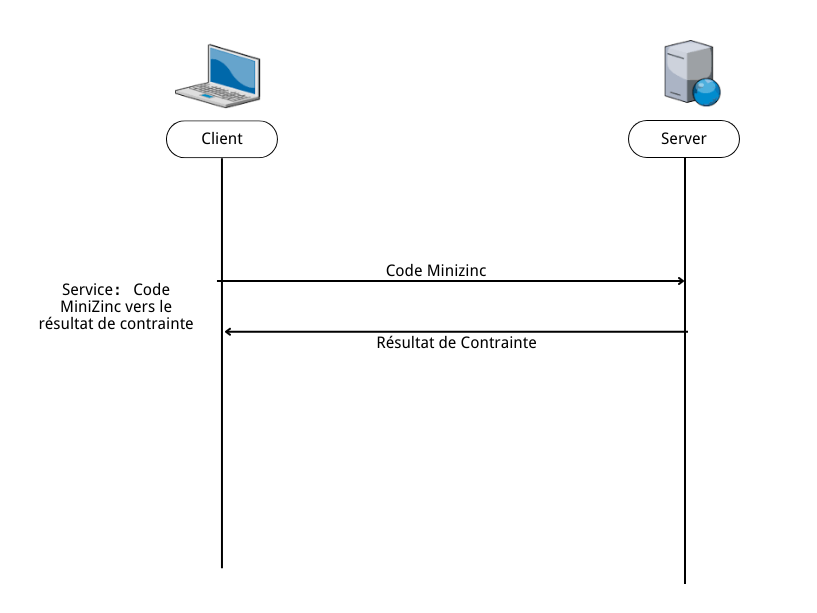
\includegraphics[scale=0.5]{Figures/CommunicationMiniZinc.png}
      \caption{Schéma de communication}
\end{figure}

\iffalse
      \hypertarget{outils-et-technologies-utilisuxe9s-1}{%
            \subsubsection{Outils et technologies
                  utilisés}\label{outils-et-technologies-utilisuxe9s-1}}

      \begin{itemize}
            \item
                  \textbf{Node.js} \cite{Node_js} : Node.js
                  permet une gestion asynchrone des opérations entrantes, ce qui permet
                  d'exécuter plusieurs opérations simultanément sans bloquer le fil
                  d'exécution principal. Par exemple, si deux requêtes sont envoyées au
                  serveur en même temps, elles seront gérées en parallèle par le
                  serveur. Ainsi, grâce à cette gestion asynchrone, Node.js permet
                  d'optimiser l'utilisation des ressources système en réduisant les
                  temps d'attente et en évitant les blocages inutiles, ce qui peut
                  augmenter l'efficacité et les performances du programme. En outre,
                  NodeJS est également connu pour son excellent support de la gestion
                  des entrées/sorties et du traitement de données en temps
                  réel.\newline  De plus, la grande quantité de packages disponible sur
                  NPM (le gestionnaire de packages de Node.js) permet de gagner beaucoup
                  de temps de développement et de faciliter notre tâche. Par example, le
                  module Child processes
                  \cite{Child_Processes} nous permet
                  d'exécuter le code MiniZinc en passant les commandes directement. Cela
                  nous permet d'éviter les restrictions du côté tout-client au niveau du
                  solveur de contraintes notamment. Enfin, un des avantages de Node.js
                  est qu'il nous permet d'utiliser le même langage de programmation que
                  le client. On s'évite ainsi les écueils autour de l'interopérabilité
                  et de la compatibilité entre deux instances codées dans des langages
                  différents.
            \item
                  \textbf{Express.js} \cite{Express_js} :
                  Express.js est une bibliothèque d'application web populaire basée sur
                  la plateforme Node.js, utilisé pour construire des applications web et
                  des API évolutives. Il fournit de nombreux middlewares, tels que
                  morgan \cite{morgan} pour enregistrer les
                  journaux de session HTTP et helmet
                  \cite{helmet} pour garantir la sécurité.
                  Avec Express.js, nous pouvons facilement ajouter des middlewares en
                  utilisant directement \texttt{app.use()} sans avoir à les ajouter
                  manuellement. De plus, Express.js dispose d'un puissant routeur qui
                  permet aux développeurs de gérer facilement les routes et de
                  construire des API REST de manière efficace. Par conséquent,
                  l'utilisation d'Express.js rend la développement plus facile et plus
                  efficace, et rend également le code plus concis. Donc il permet aux
                  développeurs de créer facilement des applications web plus rapides et
                  évolutives. Il dispose d'une plus grande communauté que les
                  bibliothèques plus jeunes, avec de nombreuses ressources et solutions
                  disponibles.
      \end{itemize}

      \newpage

      \begin{itemize}
            \item
                  \textbf{REST API} \cite{PC3R} : L'API REST
                  est un modèle de conception d'interface de programmation d'application
                  Web (API) utilisé pour fournir un accès aux ressources sur le Web. Il
                  est basé sur le protocole HTTP et utilise des requêtes et des réponses
                  HTTP pour communiquer. \newline  La conception de l'API REST est très
                  simple. Elle utilise des verbes HTTP (GET, POST, PUT, DELETE, etc.)
                  pour représenter les opérations effectuées, ainsi que des formats de
                  données standards (tels que JSON, XML) pour la transmission de
                  données. L'état des réponses est représenté sous la forme de codes
                  d'état HTTP. Par exemple, le code 200 représente le succès, le code
                  404 représente la ressource introuvable, etc.\newline  Cela permet aux
                  clients de rapidement déterminer le résultat de la réponse en fonction
                  du code d'état, sans avoir besoin de parser des informations de
                  réponse complexes. Par rapport à ``SOAP'' qui ne peut utiliser que XML
                  pour transférer des informations, l'API REST simplifie et facilite
                  l'échange de données entre les clients et les serveurs.
            \item
                  \textbf{Morgan} \cite{morgan} : Morgan est
                  un middleware JavaScript permettant d'enregistrer les journaux de
                  session HTTP. Elle peut produire des informations dans plusieurs
                  endroits (la console, les fichiers, les en-têtes HTTP\ldots) pour nous
                  aider à déboguer et à analyser le fonctionnement de leurs
                  applications. De plus, Morgan peut être facilement ajouté aux
                  applications Node.js en installant simplement les dépendances à l'aide
                  de npm et en les introduisant dans l'application à l'aide d'Express.js
                  \cite{Express_js}. Par rapport à d'autres
                  outils similaires, Morgan est plus facile à utiliser, car il ne
                  nécessite pas d'écriture de code supplémentaire. Ainsi, Morgan produit
                  une plus grande variété des cibles de sortie.
            \item
                  \textbf{Helmet} \cite{helmet} : Helmet est
                  un middleware pour les applications Node.js, conçu pour aider à
                  protéger les applications Web contre certaines attaques Web courantes.
                  De plus, l'utilisation de Helmet est très facile, en installant
                  simplement les dépendances à l'aide de npm et en les introduisant dans
                  l'application à l'aide d'Express.js
                  \cite{Express_js}. Et Helmet est un
                  middleware populaire pour Node.js, bénéficiant d'une maintenance
                  actifs de la communauté, ce qui nous permet de bénéficier facilement
                  d'aide et de support dans la communauté.
      \end{itemize}

      \hypertarget{tuxe2ches-ruxe9alisuxe9es}{%
            \subsection{Tâches réalisées}\label{tuxe2ches-ruxe9alisuxe9es}}

      \begin{itemize}
            \tightlist
            \item
                  Intégration d'un IDE similaire aux \emph{Playground} de
                  \href{https://OCaml.org/play}{OCaml} et
                  \href{https://rescript-lang.org/try}{Rescript}
            \item
                  Implémentation d'un éditeur de code supportant la syntaxe de
                  \textbf{MiniML}
            \item
                  Liaison entre le code Javascript et OCaml à l'aide de Js\_of\_OCaml
            \item
                  Implémentation de plusieurs modes de traitement du code
                  \textbf{MiniML}:

                  \begin{itemize}
                        \tightlist
                        \item
                              Affichage de l'AST MiniML
                        \item
                              Affichage de l'AST de \textbf{Call-By-Push-Value}
                        \item
                              Affichage de l'équation résultant de l'analyse statique
                        \item
                              Vers Représentation Interne \textbf{Autobill}
                  \end{itemize}
            \item
                  Remontée d'erreurs et affichage dynamique sur l'interface
            \item
                  Implémentation du solveur d'équations MiniZinc côté client
            \item
                  Mise en place d'un serveur distant manipulant les libraires OCaml du
                  projet et le solveur MiniZinc
            \item
                  Exposition du serveur avec une API REST
            \item
                  Mise en relation du client et du serveur
      \end{itemize}
\fi
\newpage

\hypertarget{miniml}{%
      \section{MiniML}\label{miniml}}

\hypertarget{description-de-miniml}{%
      \subsection{Description de MiniML}\label{description-de-miniml}}

\textbf{MiniML} émerge du choix par nos encadrants de créer un langage
fonctionnel simple et accessible pour les utilisateurs d'Autobill
servant d'abstraction à \textbf{CBPV}. Nous avons pris la décision de rendre la syntaxe MiniML parfaitement
compatible avec OCaml simplifiant les comparaisons avec d'autres outils utilisant \textbf{OCaml} en entrée.

Le développement de \textbf{MiniML} suivant les besoins de nos
encadrants celui-ci est sans effets de bord.

\hypertarget{grammaire}{%
      \subsection{Grammaire}\label{grammaire}}


\newcommand{\grammarRule}[1]{\; \textbf{<\textcolor{Blue}{#1}>} \;}
\newcommand{\grammarRuleUnSpaced}[1]{\textbf{<\textcolor{Blue}{#1}>}}
\newcommand{\nTime}[1]{\; #1\text{*} \;}
\newcommand{\nPlus}[1]{\; #1\text{+} \;}
\newcommand{\isToken}[1]{\; \textit{`\textcolor{Maroon}{#1}`} \;}
\newcommand{\isTokenLCBPV}[1]{\; \textit{`\textcolor{Green}{#1}`} \;}
\newcommand{\isRangeToken}[2]{\; \textit{`\textcolor{Maroon}{#1} - \textcolor{Maroon}{#2}`} \;}
\newcommand{\isExtentionML}[1]{ \textit{\textcolor{Orange}{#1}} \quad }

Voici la grammaire BNF du language MiniML.\
Pour des raisons de lisibilité, tous les éléments de sucre syntaxiques ne seront pas détaillés ici.\
Les extensions non compatibles avec Ocaml mais compatibles avec \textbf{Autobill} sont en \textcolor{Orange}{Orange}.

\hypertarget{Elements Nommés}{%
      \subsubsection*{Elements Nommés}\label{Elements Nommés}}

\begin{align*}
      \grammarRule{Id} ::= \quad             & \nPlus{[\isRangeToken{a}{z} \isRangeToken{A}{Z} \isRangeToken{0}{9} \isToken{\_}]} \\
      \grammarRule{ConstructeurId} ::= \quad & [\isRangeToken{A}{Z}] \grammarRule{Id}                                             \\
      \grammarRule{Vartype} ::= \quad        & \isToken{'}[\isRangeToken{a}{z}] \; \nTime{[\isRangeToken{0}{9}]}
\end{align*}

\hypertarget{programmes}{%
      \subsubsection*{Programmes}\label{programmes}}


\begin{align*}
      \grammarRule{Prog} ::= \quad & |\quad \grammarRule{Expr}                                  \\
                                   & |\quad \grammarRule{Def}  \isToken{;;}  \grammarRule{Prog}
\end{align*}

\hypertarget{definitions}{%
      \subsubsection*{Definitions}\label{definitions}}

\begin{align*}
      \grammarRule{Def} ::= \quad              & |\quad \isToken{let} \grammarRule{Id} \isToken{=} \grammarRule{Expr}                                                  \\
                                               & |\quad \isToken{type} \nTime{\grammarRuleUnSpaced{Vartype}} \grammarRule{Id} \isToken{=} \grammarRule{NewContructors} \\
      \\
      \grammarRule{NewContructors} ::=   \quad & |\quad  \grammarRule{ConstructeurId} \isToken{of} \grammarRule{Type}                                                  \\
                                               & |\quad  \grammarRule{NewContructors} \isToken{|} \grammarRule{NewContructors}                                         \\
      \isExtentionML{Debut Extension}          & |\quad \grammarRule{ConstructeurId} \isToken{of} \grammarRule{Type}  \isToken{with}  \grammarRule{ParamAssigns}       \\
      \\
      \grammarRule{ParamAssigns} ::= \quad     & |\quad \grammarRule{VarType} \isToken{=} \grammarRule{ParmExpr}                                                       \\
                                               & |\quad \grammarRule{ParamAssigns} \isToken{,} \grammarRule{ParamAssigns}                                              \\
      \grammarRule{ParmExpr} ::= \quad
                                               & |\quad \isToken{1}                                                                                                    \\
                                               & |\quad \grammarRule{VarType}                                                                                          \\
                                               & |\quad \grammarRule{ParmExpr} \isToken{+} \grammarRule{ParmExpr}                                                      \\
      \isExtentionML{Fin Extension}            & |\quad \grammarRule{ParmExpr} \isToken{*} \grammarRule{ParmExpr}                                                      \\
\end{align*}

\hypertarget{expressions}{%
      \subsubsection*{Expressions}\label{expressions}}
\begin{align*}
      \grammarRule{Litteral}  \quad ::=  \quad       & |\quad \nPlus{[\isRangeToken{0}{9}]}                                                                                                                                                  \\
                                                     & |\quad [\isToken{true}|\isToken{false}]                                                                                                                                               \\
                                                     & |\quad \isToken{(} \isToken{)}                                                                                                                                                        \\
      \\
      \grammarRule{Expr}  \quad ::=  \quad           & |\quad \grammarRule{Litteral}                                                                                                                                                         \\
                                                     & |\quad \grammarRule{Id}                                                                                                                                                               \\
                                                     & |\quad \grammarRule{UnaryOperator}  \grammarRule{Expr}                                                                                                                                \\
                                                     & |\quad  \grammarRule{Expr} \grammarRule{BinaryOperator}    \grammarRule{Expr}                                                                                                         \\
                                                     & |\quad \grammarRule{Expr}  \grammarRule{Expr}                                                                                                                                         \\
                                                     & |\quad \grammarRule{Expr} \isToken{,}  \grammarRule{Expr}                                                                                                                             \\
                                                     & |\quad \isToken{let} \grammarRule{Id} \isToken{=} \grammarRule{Expr} \isToken{in} \grammarRule{Expr}                                                                                  \\
                                                     & |\quad \isToken{fun} \grammarRule{Id} \isToken{->}  \grammarRule{Expr}                                                                                                                \\
                                                     & |\quad \isToken{fun} \isToken{rec} \grammarRule{Id} \grammarRule{Id} \isToken{->}  \grammarRule{Expr}                                                                                 \\
                                                     & |\quad \grammarRule{ConstructeurId}  \grammarRule{Expr}                                                                                                                               \\
                                                     & |\quad \isToken{match} \grammarRule{Expr} \isToken{with} \grammarRule{MatchCase}                                                                                                      \\
      \\
      \grammarRule{UnaryOperator}  \quad ::=  \quad  & \isToken{not}                                                                                                                                                                         \\
      \grammarRule{BinaryOperator}  \quad ::=  \quad & [\isToken{and} \,|\, \isToken{or} \,|\, \isToken{+} \,|\, \isToken{-} \,|\, \isToken{/} \,|\, \isToken{\%} \,|\, \isToken{*} \,|\, \isToken{<} \,|\, \isToken{>}  \,|\, \isToken{=} ] \\
\end{align*}


\hypertarget{filtrage-et-motifs}{%
      \subsubsection*{Filtrage et Motifs}\label{filtrage-et-motifs}}
\begin{align*}
      \grammarRule{MatchCase}  \quad ::=  \quad & |\quad  \grammarRule{Pattern} \isToken{->}  \grammarRule{Expr}     \\
                                                & |\quad \grammarRule{MatchCase} \isToken{|} \grammarRule{MatchCase} \\
      \\
      \grammarRule{Pattern} \quad ::=  \quad    & |\quad \grammarRule{Litteral}                                      \\
                                                & |\quad \grammarRule{Id}                                            \\
                                                & |\quad \grammarRule{Pattern}  \isToken{,} \grammarRule{Pattern}    \\
                                                & |\quad \grammarRule{ConstructeurId} \; \grammarRule{Pattern}       \\
\end{align*}


\hypertarget{types-1}{%
      \subsubsection*{Types}\label{types-1}}

\begin{align*}
      \grammarRule{Type}    \quad ::=  \quad & |\quad \grammarRule{Vartype}                              \\
                                             & |\quad \grammarRule{Id}                                   \\
                                             & |\quad \grammarRule{Type}   \grammarRule{Type}            \\
                                             & |\quad \grammarRule{Type} \isToken{->} \grammarRule{Type} \\
                                             & |\quad \grammarRule{Type} \isToken{*}  \grammarRule{Type} \\
\end{align*}

\hypertarget{call-by-push-value}{%
      \subsection{Call-By-Push-Value}\label{call-by-push-value}}

Le paradigme de traitement de langage \textbf{Call-By-Push-Value}
utilisé par \textbf{Autobill} permet à l'aide d'une seule sémantique de
traiter deux types de stratégies d'évaluation différentes, \textbf{Call
      By Value} utilisée par \textbf{OCaml} et \textbf{Call By Name} utilisée
par \textbf{Haskell} pour mettre en place l'évaluation \emph{Lazy}.

En CBPV, les valeurs et les calculs sont deux notions bien distinctes, les calculs peuvent produire et donc être réduit on dit qu'ils "font";
tandis que les valeurs sont des contenants et ne peuvent pas être réduit on dit qu'ils "sont".
Lorsqu'on effectue la traduction depuis une autre sémantique, nous devons donc décider comment et quand nos calculs vont être effectués.

Dans le cadre de ce projet, 3 constructions de LCBPV nous intéressent particulièrement, les \textbf{Closure}, les \textbf{Thunks} et les \textbf{Methods}.
\begin{itemize}
      \item
            Les \textbf{Thunks} sont des expressions non évaluées, ils sont utilisés pour représenter un calcul qui n'a pas encore été effectué.
            On peut donc les voir comme des lambdas sans arguments.
            Pour forcer l'évaluation d'un \textbf{Thunk} il suffit d'utiliser l'instruction  \textbf{force}.
      \item
            Les \textbf{Closures} qui permettent de capturer un environnement et une expression et de les lier.
      \item
            Les \textbf{Methods} qui dans notre cas permet de définir des calculs à effectuer avec des arguments.
\end{itemize}
Pour plus d'informations sur LCBPV sa syntaxe, sa sémantique et ses constructions, vous pouvez vous référer à l'annexe de ce rapport.

\hypertarget{semantique-de-traduction}{%
      \subsection{Semantique de traduction}\label{semantique-de-traduction}}

Puisque MiniML est un language \emph{Call By Value}, ici nous décidons que toute traduction nécessitant le passage par la notion de calculs dans CBPV forcera immédiatement l'évaluation de ceux-ci.
Permettant ainsi une équivalence parfaite entre tout comportement de MiniML traduit en LCBPV.

Pour décrire la traduction de MiniML en LCBPV, nous allons opter pour une traduction de syntaxe concrète à syntaxe concrète.
Vous trouverez ci-dessous tous les cas d'intérêts de la traduction.

\newcommand{\translateNode}[2]{\llbracket #1 \rrbracket_{#2}}
\newcommand{\translateResult}[1]{\llbracket #1 \rrbracket}
\newcommand{\isElemMiniML}[1]{\; \textcolor{Maroon}{#1} \;}
\newcommand{\isElemLCBPV}[1]{\textcolor{ForestGreen}{#1}}
\newcommand{\spaced}[1]{\; #1 \;}
\newcommand{\Tab}{\quad \quad \quad \quad \quad \quad \;}

\pagebreak
\hypertarget{notation}{%
      \subsubsection*{Notation}\label{notation}}
$ \translateNode{let \; v \; = \; e_1 \; in \; e_2}{Expr}  \rightarrow let \; v = \; \translateResult{e_1} \; in \; \translateResult{e_2}$
\begin{itemize}
      \tightlist
      \item
            $\translateNode{\_}{Expr}  \rightarrow $ est la traduction d'un noeud expr du langage MiniML vers le langage LCBPV
            \begin{itemize}
                  \tightlist
                  \item
                        À l'interieur des $\translateResult{}$, nous trouvons les elements propre au langage MiniML qui sont traduit vers le langage LCBPV.
                  \item
                        À l'exterieur des $\translateResult{}$, nous trouvons les elements propre au langage LCBPV.
            \end{itemize}
      \item
            $X_n$ est le n-ième sous-noeud de l'arbre de syntaxe abstrait. \newline
            Selon les cas $X$ peut être :
            \begin{itemize}
                  \tightlist
                  \item
                        $e$ pour les expressions
                  \item
                        $p$ pour les motifs
                  \item
                        $t$ pour les types
                  \item
                        $d$ pour les définitions
                        \begin{itemize}
                              \tightlist
                              \item
                                    $dc$ pour les définitions de constructeurs
                        \end{itemize}
                  \item
                        $v$ pour les elements nommées
                  \item
                        $op$ pour les opérateurs
                  \item
                        $l$ pour les litteraux
            \end{itemize}
      \item
            $X_1 \dots X_n$ est la liste des sous-noeuds de type $X$ allant de $1$ à $n$
\end{itemize}


\hypertarget{programmes-1}{%
      \subsubsection*{Programmes}\label{programmes-1}}

Un programme MiniML est une suite de taille arbitraire de définitions suivie d'une expression.

\begin{align*}
      \translateNode{d_1 \dots d_n \, e}{Prog} \rightarrow \translateResult{d_1 \dots d_n}\; return \; \translateResult{e}
\end{align*}

\subsubsection*{Définitions}\label{def}

On définit l'opération de traduction \(\translateNode{\_}{Def}\) selon les cas de construction
des définitions précisées par la règle de grammaire : \grammarRule{Def}

On distingue deux noeuds du type \grammarRule{Def}:
\begin{itemize}
      \tightlist
      \item
            Les définitions de \textbf{Variables Globales},
      \item
            Les définitions de \textbf{Types}.
\end{itemize}
\begin{align*}
      \text{(VARDEF)}  \quad & \translateNode{let \, v \, = \, e}{Def} \rightarrow   let \, v \, = \; \translateResult{e}       \\
      \text{(TYPDEF) } \quad & \translateNode{type \, \, v_1 \dots v_N \, = \, dc_1 \dots  dc_N}{Def}                           \\
      \rightarrow \;         & data \translateResult{v_1} (\translateResult{\dots v_N} : +) = \translateResult{dc_1 \dots dc_N} \\
\end{align*}
\subsubsection*{Définitions de Constructeurs}\label{defConstruct} \hfill \break

On définit l'opération de traduction \(\translateNode{\_}{DefContructors}\) selon les cas de construction précisées par la règle de grammaire : \grammarRule{NewContructors}

On distingue deux noeuds du type \grammarRule{NewContructors}:
\begin{itemize}
      \tightlist
      \item
            Les définitions de \textbf{Constructeurs Classiques} qui sont compatibles avec OcamL.
      \item
            Les définitions de \textbf{Constructeurs Equationnels} qui sont une extension spécifique pour \textbf{Autobill} incompatible avec OcamL et dont la traduction n'est pas encore totalement définie.
\end{itemize}
\begin{align*}
      \text{(MLCONSTRUCTDEF)} \quad & \translateNode{v \; of \; t}{DefContructors}   \rightarrow   v\translateResult{t} \\
\end{align*}

\subsubsection*{Types}\label{types-2}

On définit l'opération de traduction \(\translateNode{\_}{Type}\) selon les cas de construction
des types précisées par la règle de grammaire : \grammarRule{Type}

On distingue 4 noeuds du type $Type$:
\begin{itemize}
      \tightlist
      \item
            Les \textbf{Variables de types}.
      \item
            Les \textbf{Applications de types}.
      \item
            Les \textbf{Lambda}.
      \item
            Les \textbf{Tuples}.
\end{itemize}
\begin{align*}
      \text{(TVAR) }  & \translateNode{v}{Type} \rightarrow  v                                                                                          \\
      \text{(TAPP) }  & \translateNode{t_1 t_2}{Type} \rightarrow  \translateResult{t_1} \, \translateResult{t_2}                                       \\
      \text{(TCLOS) } & \translateNode{t_1 \text{->} t_2}{Type} \rightarrow  Exp (Fun\translateResult{t_1} \, \text{->} \, Thunk\translateResult{t_2} ) \\
      \text{(TTUPLE)} & \translateNode{t_1 * t_2}{Type} \rightarrow  \translateResult{t_1} \,  \, \translateResult{t_2}
\end{align*}

\subsubsection*{Expressions}\label{exprs}

On définit l'opération de traduction \(\translateNode{\_}{Expr}\) selon les cas de construction
des expressions précisées par la règle de grammaire : \grammarRule{Expr}

On distingue 8 noeuds d'intérêts du type \grammarRule{Expr}:
\begin{itemize}
      \tightlist
      \item
            Les \textbf{Tuples}.
      \item
            Les \textbf{Appels de fonctions}.
      \item
            Les \textbf{Fixation}.
      \item
            Les \textbf{Lambda}.
      \item
            Les \textbf{Fonctions Recursive}.
      \item
            Les \textbf{Constructions}.
      \item
            Les \textbf{Correspondance de motifs}.
      \item
            Les \textbf{Appels d'operateurs}.
\end{itemize}
\textbf{Note:} On ne prend pas en compte les \textbf{Littéraux} et les \textbf{Variables} dans ce descriptif car leurs traductions sont directes.
\begin{align*}
      \text{(BINARY)} \quad    & \translateNode{e_1 \, op \, e_2}{Expr} \rightarrow \translateResult{e_1} \, \, op \, \, \translateResult{e_2}                                                                  \\
      \text{(UNARY)} \quad     & \translateNode{op \, e}{Expr} \rightarrow op \, \, \translateResult{e}                                                                                                         \\
      \text{(TUPLE)} \quad     & \translateNode{e_1 \, , \, e_2}{Expr} \rightarrow \text{Tuple}(\translateResult{e_1} \, \, \translateResult{e_2})                                                              \\
      \text{(LAMBDA)} \quad    & \translateNode{fun \, v \, \rightarrow \, e}{Expr}    \rightarrow  exp(  \; get \; | \; call(v) \; \text{->}  \; thunk\translateResult{e}  )                                   \\
      \text{(FUN REC)} \quad   & \translateNode{fun \, rec \, v_1 \, v_2 \rightarrow \, e}{Expr}      \rightarrow exp( \; rec \; v_1 \; is \; get \; | \; call(v_2) \; \text{->}  \; thunk\translateResult{e} ) \\
      \text{(CALL)} \quad      & \translateNode{e_1 e_2}{Expr}     \rightarrow  \{                                                                                                                              \\
                               & \Tab open \; exp \; v_1  = \translateResult{e_1}                                                                                                                               \\
                               & \Tab force \; thunk(v_2) = (v_1).call\translateResult{e_2}                                                                                                                     \\
                               & \Tab return \; v_2                                                                                                                                                             \\
                               & \}                                                                                                                                                                             \\
      \text{(BIND)} \quad      & \translateNode{let \; v \; = \; e_1 \; in \; e_2}{Expr}  \rightarrow  \{                                                                                                       \\
                               & \Tab let \; v = \translateResult{e_1}                                                                                                                                          \\
                               & \Tab return \;\translateResult{e_2}                                                                                                                                            \\
                               & \}                                                                                                                                                                             \\
      \text{(CONSTRUCT)} \quad & \translateNode{v \, e}{Expr} \rightarrow v\translateResult{e}                                                                                                                  \\
      \text{(MATCH)} \quad     & \translateNode{match \, e \, with \, p_1 \dots p_N }{Expr}\rightarrow  match \, \translateResult{e} \, with \, \translateResult{p_1} \dots \translateResult{p_N} \; end        \\
\end{align*}

Les cas de traductions les plus intéressants sont ceux des \textbf{Fonctions} et les \textbf{Appels de Fonctions}.
La traduction d'une fonction se déroule ainsi:
\begin{enumerate}
      \tightlist
      \item
            À l'aide de l'instruction \textbf{get} on crée une méthode \textbf{call} qui prend en paramètre un argument.
      \item
            Ensuite dans le corps de cette méthode on crée un \textbf{Thunk} qui contient la traduction du corps de la fonction.
      \item
            Puis on crée une \textbf{Closure} qui contient la méthode ainsi créée et son environnement.
\end{enumerate}
Au vu de la traduction des fonctions, on peut en déduire la traduction des appels:
\begin{enumerate}
      \tightlist
      \item
            On ouvre la \textbf{Closure} de la fonction.
            Pour récupérer la méthode \textbf{call} et l'environnement.
      \item
            On applique la méthode \textbf{call} sur l'argument fourni au moment de l'appel.
            Pour récupérer un \textbf{Thunk} sur le corps de la fonction  avec l'environnement enrichi de l'argument.
      \item
            On force le \textbf{Thunk} ainsi obtenu pour avoir l'évaluation immédiate du corps de la fonction.
\end{enumerate}

\subsubsection*{Motifs et Filtrage}\label{motifs-et-filtrage}

On définit l'opération de traduction \(\translateNode{\_}{Case}\) selon les cas de construction
des expressions précisées par la règle de grammaire : \grammarRule{MatchCase}

On distingue 4 noeuds d'intérêt du type \grammarRule{MatchCase}:
\begin{itemize}
      \tightlist
      \item
            Les patterns sur \textbf{Litteraux}.
      \item
            Les patterns sur \textbf{Variables}.
      \item
            Les patterns sur \textbf{Tuple}.
      \item
            Les patterns sur \textbf{Constructeurs}.
\end{itemize}

\begin{align*}
      \text{(PATTERN LIT)} \quad    & \translateNode{l \; \text{->} \; e}{MatchCase} \rightarrow \translateResult{l} \; \text{->} \; \translateResult{e}                \\
      \text{(PATTERN VAR)} \quad    & \translateNode{v \; \text{->} \; e}{MatchCase} \rightarrow v \; \text{->} \; \translateResult{e}                                  \\
      \text{(PATTERN TUPLE)} \quad  & \translateNode{v_1 \, , \, v_2 \, \text{->} \; e}{MatchCase} \rightarrow Tuple(v_1 \, \, v_2) \; \text{->} \; \translateResult{e} \\
      \text{(PATTERN CONSTR)} \quad & \translateNode{v_1 \, v_2 \, \text{->} \; e}{MatchCase} \rightarrow v_1 \, v_2 \; \text{->} \; \translateResult{e}                \\
\end{align*}

On notera que la traduction des patterns ne prend pas en compte les patterns profonds, c'est-à-dire les patterns imbriqués dans d'autres patterns.
En effet, les patterns profonds ne sont pas encore supportés par le language cible.


\hypertarget{Implémentation}{%
      \subsection{Implémentation}\label{Implementation}}
Dans le cadre de ce projet, MiniML dispose d'une implémentation écrite en OCaml nous avons utilisé ce langage pour deux raisons principales.
Permettre une meilleure intégration avec autobill qui est écrit dans le même language ce qui a permis d'unifier la gestion d'erreurs
et la seconde raison est la double compatibilité avec les deux architectures cibles.
Cette forte proximité avec le code d'autobill a rendu possible la traduction non pas de syntaxe concrète à syntaxe concrète comme décrite ci-dessus mais de syntaxe abstraite à syntaxe abstraite.
Nous épargnant ainsi une nouvelle étape d'analyse syntaxique.
Deux autres divergences avec la spécification est l'utilisation d'une fonction de traduction récursive terminale par souci d'optimisation et l'ajout de nombreux sucres syntaxiques pour faciliter l'écriture de programmes Mini Ml.


\hypertarget{conclusion}{%
      \section{Conclusion}\label{conclusion}}
\hypertarget{conclusion}{%
  \subsection{Avancement du projet}\label{Avancement du Projet}}

L'objective de notre projet STL est construire un pipeline du MiniML à la résolution de contrainte ( MiniML $\rightarrow$ LCBPV $\rightarrow$ Autobill $\rightarrow$ Équation $\rightarrow$ Résolution). Dans la partie MiniML, nous avons utilisé MiniML pour rédiger le lexer et le parser pour Autobill, ainsi que pour finir la traduction de MiniML vers CBPV. Ce qui complète la partie MiniML $\rightarrow$ LCBPV $\rightarrow$ Autobill dans la pipeline, et produire l'entrée d'Autobill pour faire l'analyse à la suite. Parallèlement, nous avons développé une interface web en utilisant React et NodeJS, en mode client-seulement et de client-server. Le service "MiniML $\rightarrow$ LCBPV" du interface présente de manière satisfaisante les résultats des étapes précédentes. Cet interface utilise également Minizinc pour analyser l'équation de l'analyse statique, afin d'obtenir les bornes sur la consommation de mémoire du programme dans le service "Équation $\rightarrow$ Solution". Ce qui complète la partie Équation $\rightarrow$ Résolution de la pipeline. Nous avons utilisé quelque programmes pour comparer  les resultats obtenu par côte client et côte server, et nous avons eu le même resultat.\\

Cependant, la partie Autobill $\rightarrow$ Équation est toujours en progress. H.Suzanne travaille encore sur les détails de l'Autobill afin de obtenir l'équation parfaitement. Donc nous ne pouvons pas finalement construire la pipeline entière, pour obtenire le borne de mémoire à patir de la programme MiniML. Mais notre avancement de ce projet STL a pu répondre à la plupart des besoins de la section 1 du rapport.\\
      
La réalisation de cette interface a fait intervenir un large panel de
sujets en lien avec la formation du Master d'informatique STL et mis à
profit les connaissances acquises lors de ce semestre. En premier lieu,
le cours d'analyse de programme statique
\protect\hyperlink{ref-APS}{{[}24{]}} pour toute la partie MiniML et le
processus de transformation vers CBPV. Puis, les cours de programmation
concurrente répartie, réactive et réticulaire
\protect\hyperlink{ref-PC3R}{{[}22{]}}, notamment pour la partie
réticulaire et l'architecture d'applications Web modernes.\\

\subsection{Difficulté rencontré}\label{Difficulté rencontré}}

Nous avons également rencontré quelques difficultés pour faire avancer le projet. Tout d'abord, nous n'avons pas été en mesure de construire un pipeline MiniML $\rightarrow$ LCBPV $\rightarrow$ Autobill $\rightarrow$ Équation $\rightarrow$ Résolution, avec le lien Autobill $\rightarrow$ Équation est toujours en progress. Et finalement nous ne pouvons pas comparer notre solution avec celle de J.Hoffmann et l'interface de RAML. Deuxièmement, notre projet avance en parallèle avec H.Suzanne et nous devons être totalement concentré dans le recherche, et nous accommoder mutuellement des progrès réalisés par les deux parties. Aussi nous avons plusieurs projets en même temps, et nous avons eu beaucoup de challenge de gestion de temps. \\

\subsection{Ce qu'on a appris}\label{Ce qu'on a appris}}
Cependant, ce projet nous a beaucoup apporté. Tout d'abord, notre capacité à écrire du code a été améliorée et nous avons acquis une meilleure compréhension des principes de compilation et de la composition des langages de programmation. Deuxièmement, nous avons lu un certain nombre d'articles dans lesquels nous avons appris la grande contribution de J.Hoffmann à l'étude de l'analyse automatique des ressources amorties et les principes de call-by-push-value. Notre capacité à gérer le temps et à travailler en mode multiple-threads, comme mentionné ci-dessus, a également été améliorée.\\

\subsection{Pour aller plus loin...}\label{Pour aller plus loin...}}
Le projet est à un stade d'avancement satisfaisant. Autobill étant
encore en phase expérimentale, celui-ci est alimenté continuellement de
nouveautés et corrections que l'on doit intégrer. Dans le futur, quand nous avons avoir une pipeline entière, il serait intéressant à titre de démonstration de comparer notre solution avec celle de Jan Hoffmann et l'interface de RAML
\protect\hyperlink{ref-RAML}{{[}3{]}} et deployer notre interface Web en ligne.

\newpage
\bibliographystyle{ieeetr}
\bibliography{biblio}{}

\newpage

\section*{Annexe}\label{annexe}
\addcontentsline{toc}{section}{\protect\numberline{}Annexe}%

% Add ',fontsize=\small' for more characters per line
\newenvironment{Shaded}{}{}
\newcommand{\AlertTok}[1]{\textcolor[rgb]{1.00,0.00,0.00}{\textbf{#1}}}
\newcommand{\AnnotationTok}[1]{\textcolor[rgb]{0.38,0.63,0.69}{\textbf{\textit{#1}}}}
\newcommand{\AttributeTok}[1]{\textcolor[rgb]{0.49,0.56,0.16}{#1}}
\newcommand{\BaseNTok}[1]{\textcolor[rgb]{0.25,0.63,0.44}{#1}}
\newcommand{\BuiltInTok}[1]{\textcolor[rgb]{0.00,0.50,0.00}{#1}}
\newcommand{\CharTok}[1]{\textcolor[rgb]{0.25,0.44,0.63}{#1}}
\newcommand{\CommentTok}[1]{\textcolor[rgb]{0.38,0.63,0.69}{\textit{#1}}}
\newcommand{\CommentVarTok}[1]{\textcolor[rgb]{0.38,0.63,0.69}{\textbf{\textit{#1}}}}
\newcommand{\ConstantTok}[1]{\textcolor[rgb]{0.53,0.00,0.00}{#1}}
\newcommand{\ControlFlowTok}[1]{\textcolor[rgb]{0.00,0.44,0.13}{\textbf{#1}}}
\newcommand{\DataTypeTok}[1]{\textcolor[rgb]{0.56,0.13,0.00}{#1}}
\newcommand{\DecValTok}[1]{\textcolor[rgb]{0.25,0.63,0.44}{#1}}
\newcommand{\DocumentationTok}[1]{\textcolor[rgb]{0.73,0.13,0.13}{\textit{#1}}}
\newcommand{\ErrorTok}[1]{\textcolor[rgb]{1.00,0.00,0.00}{\textbf{#1}}}
\newcommand{\ExtensionTok}[1]{#1}
\newcommand{\FloatTok}[1]{\textcolor[rgb]{0.25,0.63,0.44}{#1}}
\newcommand{\FunctionTok}[1]{\textcolor[rgb]{0.02,0.16,0.49}{#1}}
\newcommand{\ImportTok}[1]{\textcolor[rgb]{0.00,0.50,0.00}{\textbf{#1}}}
\newcommand{\InformationTok}[1]{\textcolor[rgb]{0.38,0.63,0.69}{\textbf{\textit{#1}}}}
\newcommand{\KeywordTok}[1]{\textcolor[rgb]{0.00,0.44,0.13}{\textbf{#1}}}
\newcommand{\NormalTok}[1]{#1}
\newcommand{\OperatorTok}[1]{\textcolor[rgb]{0.40,0.40,0.40}{#1}}
\newcommand{\OtherTok}[1]{\textcolor[rgb]{0.00,0.44,0.13}{#1}}
\newcommand{\PreprocessorTok}[1]{\textcolor[rgb]{0.74,0.48,0.00}{#1}}
\newcommand{\RegionMarkerTok}[1]{#1}
\newcommand{\SpecialCharTok}[1]{\textcolor[rgb]{0.25,0.44,0.63}{#1}}
\newcommand{\SpecialStringTok}[1]{\textcolor[rgb]{0.73,0.40,0.53}{#1}}
\newcommand{\StringTok}[1]{\textcolor[rgb]{0.25,0.44,0.63}{#1}}
\newcommand{\VariableTok}[1]{\textcolor[rgb]{0.10,0.09,0.49}{#1}}
\newcommand{\VerbatimStringTok}[1]{\textcolor[rgb]{0.25,0.44,0.63}{#1}}
\newcommand{\WarningTok}[1]{\textcolor[rgb]{0.38,0.63,0.69}{\textbf{\textit{#1}}}}

\hypertarget{syntaxe-et-suxe9mantique-informelle-de-ux3bb-cbpv}{%
      \subsection*{Syntaxe et sémantique informelle de
            LCBPV}\label{syntaxe-et-suxe9mantique-informelle-de-ux3bb-cbpv}}

\hypertarget{call-by-push-value-en-bref}{%
      \subsubsection*{Call-By-Push-Value En
            Bref}\label{call-by-push-value-en-bref}}

Le langage $\lambda$-CBPV (``lambda-call-by-push-value'', ou juste LCBPV pour
les intimes) est une réprésentation intermédiaire de haut niveau, dans
laquel on peut compiler les langages à la ML (avec évaluation stricte),
ou à la Haskell (avec évaluation paresseuse), ou mélanger les deux pour
compiler des fonctionalités avancées (comme certaines concept de
programmation objets).

Dans LCBPV, on a des valeurs et des calculs. Les valeurs \emph{sont} des
choses mais de font rien, les calculs \emph{font} des choses mais ne
contiennent pas de données. On a donc deux \emph{sortes} de type: si
\texttt{T} est type de valeur, on le défini comme \texttt{T\ :\ +} , et
de même, \texttt{T\ :\ -} est un type de calcul. Pour aider la
compréhension, quand \texttt{T} est un type de valeur, on le notera
parfois \texttt{T+}, et \texttt{T-} si c'est un type de calcul.

\hypertarget{les-types-de-valeurs}{%
      \subsubsection*{Les types de valeurs}\label{les-types-de-valeurs}}

\hypertarget{les-entiers}{%
      \paragraph*{les entiers}\label{les-entiers}}

Classique. On les écrits en base 10, avec un `-' devant pour les
négatifs. On dispose des opérations classiques: addition, substraction,
division euclidienne, reste, et négation. On peut tester pour l'égalité
et l'ordre. Le type de valeur des entier est \texttt{Int\ :\ +}

\begin{verbatim}
0 1 2 3530530899 -2 -4343  (littéraux)
1+1 2-2 3*3 4*4 -5         (opérations)
6==6 7<7 8=<8 (tests)
\end{verbatim}

\hypertarget{les-booluxe9ens}{%
      \paragraph*{Les booléens}\label{les-booluxe9ens}}

Encore classique. \texttt{true}, \texttt{false}, \texttt{and},
\texttt{or} et \texttt{not}. Le type de valeur des booléens est
\texttt{Bool\ :\ +}

\begin{verbatim}
true false 
&& || ! 
\end{verbatim}

On a un if/then/else:

\begin{verbatim}
if 1>0 then 45 else 422 
\end{verbatim}

\hypertarget{les-tuples}{%
      \paragraph*{Les tuples}\label{les-tuples}}

On les note \texttt{tuple(e\_1,\ ...,\ e\_n)}, et ils ont le type
\texttt{Tuple(T\_1+,\ ...,\ T\_n+)}. Chacun des \texttt{n} composant est
une valeur \texttt{e\_i\ :\ T\_i\ :\ +}. Le 0-uplet/tuple vide est noté
\texttt{unit()} de type de valeur\texttt{Unit}. On accède aux composants
\texttt{e\_1},\ldots,\texttt{e\_n} des tuples par pattern matching:

\begin{verbatim}
match e_tuple with
 | tuple(x_1, ..., x_n) -> ... 
end
\end{verbatim}

\hypertarget{les-types-sommes}{%
      \paragraph*{Les types sommes}\label{les-types-sommes}}

Les sommes binaires on le type de valeur \texttt{Sum(T+,U+)\ :\ +}. Ces
deux constructeurs sont
\texttt{inj\{1,2\}\ :\ T\ -\textgreater{}\ sum(T,U)} et
\texttt{inj\{2,2\}\ :\ U+\ -\textgreater{}\ Sum(T+,U+)}. En général, on
peut faire des sommes avec \emph{n} types \texttt{T\_1+,\ ...,\ T\_n+}.
On note le type de valeurs correspondant
\texttt{Sum(T\_1+,\ ...,T\_n+)\ :\ +} et on a des constructeurs
\texttt{inj\{i,n\}} pour tout \emph{i} entre 1 et \emph{n}. On peut
pattern matcher sur les sommes:

\begin{verbatim}
match e_sum with
  | inj{1,n}(x) -> ...
  | inj{2,n}(x) -> ...
  ...
  | inj{n,n} -> ...
end
\end{verbatim}

\hypertarget{duxe9finir-des-types-de-valeurs}{%
      \paragraph*{Définir des types de
            valeurs}\label{duxe9finir-des-types-de-valeurs}}

On peut, comme en OCaml, définir des types par cas. Par exemple, le type
des listes et le type option sont définis de la manière suivante:

\begin{verbatim}
data List(A : +) =
  | nil()
  | cons(A, List(A));

data Option(A : +) =
  | none()
  | some(A);
\end{verbatim}

On peut alors créer des listes en utilisant les constructeurs
\texttt{cons} et \texttt{nil}, par exemple, la liste {[}1,2,3{]} sera
encodée par \texttt{cons(1,cons(3,cons(3,nil)))}. On peut aussi faire du
fitrage par motif sur les listes. Par exemple, si on a une liste
d'entiers \texttt{l}, l'expression ci-dessous renvoit la tête de la
liste dans un type option.

\begin{verbatim}
match l with 
  | nil() -> {return none()}
  | cons(h,t) -> {return some(h)}
end 
\end{verbatim}

\hypertarget{les-blocs-thunks-et-fermetures}{%
      \subsubsection*{Les blocs, thunks, et
            fermetures}\label{les-blocs-thunks-et-fermetures}}

\hypertarget{blocs}{%
      \paragraph*{Blocs}\label{blocs}}

LCBPV utilise des blocs pour séquencer les opérations. Un bloc est une
séquence d'instruction, séparées par un point-virgule, et terminé par un
\texttt{return\ e} qui évalue \texttt{e} et renvoie et renvoie la valeur
correspondante. On a trois instructions: \texttt{let\ open\ force}. La
première est \texttt{let\ x\ =\ e;}, elle évalue \texttt{e}, et affecte
le résulat à \texttt{x}. \texttt{x} est en portée dans les instruction
suivantes dans le bloc et dans l'expression de retour. Par exemple:

\begin{verbatim}
let x = 2+2;
let y = 3+1;
return x + y
\end{verbatim}

On peut remplacer une expression par bloc avec des allocades. C'est à
dire, les expressions \texttt{e}, \texttt{\{return\ e\}}, et
\texttt{\{let\ x\ =\ e;\ return\ x\}} sont interchangeables. On va
maintenant voir \texttt{force} et \texttt{open}, qui gèrent les
\emph{thunks} et les \emph{fermetures}.

\hypertarget{les-thunks}{%
      \paragraph*{Les thunks}\label{les-thunks}}

Quand un calcul renvoie une valeur, il la renvoi encapsulée dans un
calcul nommé \emph{thunk} et noté \texttt{thunk(e)}, où est une
expression quelqueonque qui renvoie une valeur. Il faut \emph{forcer} le
thunk avec \texttt{force\ x\ =\ thunk(e)} pour calculer effectivement la
valeur de \texttt{e}, et l'affecter à \texttt{x}. Pour l'exemple,
comparez les deux fragments de code suivants, qui calculent différement
le même résultat. Dans le premier, on calcule 2+2 avant de calculer 3+1,
et dans le second on calcule 3+1 en premier et 2+2 après.

\begin{verbatim}
// fragment 1:
let x = 2+2;
let y = 3+1;
return x + y 
  
//fragment 2:
let x = thunk(2+2);
let y = thunk(3+1);
force thunk(y') = y;
force thunk(x') = x;
return x'+y'
\end{verbatim}

Si une expression \texttt{e\ :\ T\ :\ +} renvoie une valeur de type de
valeur \texttt{T}, alors le thunk \texttt{thunk(e)\ :\ Thunk(T)\ :\ -}
est une valeur de type de calcul \texttt{Thunk(T)}

\hypertarget{les-fermetures}{%
      \paragraph*{Les fermetures}\label{les-fermetures}}

Comme les thunks qui sont des calculent qui renvoient une valeur après
évaluation, on peut créer des valeurs qui stockent un calcul avant son
évaluation. si on a un calcul \texttt{f}, on peut le mettre dans une
\emph{fermeture} \texttt{closure(f)} qui bloque son évaluation et stocke
les valeurs de ses variables libres. Quand on \emph{ouvre} la fermeture
avec \texttt{open\ g\ =\ closure(f)}, on assigne \texttt{g=f} et on
remet les valeurs dont \texttt{f} dépend sur la pile. On peut alors
accéder à \texttt{g} correctment (sans segfault).

Par exemple, dans le code suivant, un créé une fermeture sur un calcul
qui renvoi un entier. Comme les entiers sont des valeurs, on créé une
fermeture autour d'un trunk qui renvoi un entier. On voit que quand on
définit un calcul, on peut évaluer les calculs en plusieurs morceaux:
quand ils sont définis, quand on ouvre leur fermeture, et quand on les
force.

\begin{verbatim}
// Au début, je n'ai pas encore évalué `a=2+2` ni `b=3+1`
let f = {

  let a = 2+2;
  // Ici, j'ai évalué 'a' mais pas `b`
    
  // la fermeture capture la variable `a=4` qui est libre dans son corps 
  return closure({
  
      // ce bloc est bloqué par la fermeture
      let b = 3+1;
      return thunk(a+b)
  })
};
  
// Ici, je n'ai toutjours pas évalué `b`
open closure(f') = f;
// Après l'ouverture de `f`, `b` est évalué et on a assigné `f' = thunk(a+b)` 
  
// Puis on force le thunk pour évaluer `a+b` et récupérer 8
force thunk(x) = f';
return x
\end{verbatim}

Si \texttt{e\ :\ T\ :\ -} est une expression qui renvoie un calcul de
type \texttt{T}, alors \texttt{closure(e)\ =\ Closure(T)\ :\ +} est une
valeur de type de valeur \texttt{Closure(T)}

\hypertarget{les-autres-types-de-calculs}{%
      \subsubsection*{Les autres types de
            calculs}\label{les-autres-types-de-calculs}}

\hypertarget{les-fonctions}{%
      \paragraph*{Les fonctions}\label{les-fonctions}}

Les fonctions en LCBPV sont des calculs. Comme en Java ou C++, on les
réprésente par des ``objets'' avec une méthode \texttt{call}. Par
exemple, la fonction ``f : x → 2x+3'' sera écrite et appelée de la
manière suivante. Notons que les fonctions qui renvoient des types de
valeurs doivent encapsuler leur valeur de retour dans un thunk, et qu'il
faut forcer le thunk pour terminer l'appel.

\begin{verbatim}
// `y` est défini comme un calcul, avec une méthode `call`:
let f = get 
    | call(x) -> thunk(2 * x + 3)
  end;
  
// `y` est un thunk qui calcule "f(1)". On a pas encore évalué f !
let y = f.call(1);

// Ici on calcule l'appel "f(1)", qui renvoie 2*1+3 = 5
force thunk(z) = y;

return z // on renvoie z = 5
\end{verbatim}

Le type des fonctions est
\texttt{Fun(T\_1+,\ ...,\ T\_n+)\ -\textgreater{}\ T-}, avec chaque
argument un type de valeur et le résultat un type de calcul. Les
fonctions en LCBPV ne sont pas currifiés. Une fontion de type
\texttt{Fun(A+,\ B+)\ -\textgreater{}\ C-} doit recevoir ces deux
arguments simultanément. Cette fonction, currifiée, serait de type
\texttt{Fun(A+)\ -\textgreater{}\ Fun(B+)\ -\textgreater{}\ C-}, ou
encore
\texttt{Fun(A+)\ -\textgreater{}\ Thunk(Closure(Fun(B+)\ -\textgreater{}\ C-))}.

\hypertarget{les-paires-paresseuses}{%
      \paragraph*{Les ``paires
            paresseuses''}\label{les-paires-paresseuses}}

Les paires paresseuses sont des objets avec plusieurs méthodes qui
renvoient chacune un type différent. Au final, seul(s) le(s) élément(s)
accédé(s) sont effectivement calculées, d'où le coté paresseux. Si on a
une paire paresseuse \texttt{p} avec \emph{n}, éléments, on appele la
méthode \texttt{p.proj\{i,n\}()} pour sélectionner le \emph{i}-ème.
Notons que qu'aucune des méthodes ne prend d'arguments, et qu'il faut
forcer le thunk pour effectivement calculer le \emph{i}-ème élément.

On défini une paire paresseuse en spécifiant chacune des méthodes
\texttt{proj\{i,n\}} dans une clause \texttt{get\ ...\ end} comme pour
les functions:

\begin{verbatim}
let douzaines = get
  | proj{1,3}() -> 12
  | proj{2,3}() -> 24
  | proj{3,3}() -> 36
end;

force thunk(x) = douzaine.proj{1,3}();

return x // renvoie 12
\end{verbatim}

\hypertarget{duxe9finir-des-types-de-calculs}{%
      \paragraph*{Définir des types de
            calculs}\label{duxe9finir-des-types-de-calculs}}

On peut aussi définir des types de calcul au cas-par-cas, c'est à dire
en définissant chaque méthode. Par exemple, on peut définir le type des
itérateurs sur les listes de la manière suivante: un itérateur est un
objet avec deux méthodes, une qui consome un élément de liste et renoie
un nouvel itérateur, et une second qui termine l'itération quand on
croise \texttt{nil()}. On définit alors un type \texttt{Iter(A,\ B)} qui
consome des listes de type \texttt{A} et renvoi un \texttt{B}. La
méthode \texttt{use\_nil()} renvoie une thunk sur le \texttt{B} final,
et \texttt{use\_cons} prend un \texttt{A} et renvoi un
\texttt{Iter(A,B)}. Notons que comme \texttt{Iter(A,B)\ :\ -} est un
type de calcul, on a pas besoin de renvoyer un thunk dans
\texttt{use\_cons}.

\begin{verbatim}
comput Iter(A : +, B : +) =
  | use_nil() -> Thunk(B)
  | use_cons(A) -> Iter(A,B);
\end{verbatim}

On définit souvent les itérateurs par récurrence, et on vera cela plus
bas.

\hypertarget{le-reste-des-fonctionalituxe9s}{%
      \subsubsection*{Le reste des
            fonctionalités}\label{le-reste-des-fonctionalituxe9s}}

\hypertarget{duxe9finitions-ruxe9cursives}{%
      \paragraph*{Définitions
            récursives}\label{duxe9finitions-ruxe9cursives}}

On peut définir des calculs récursifs avec le constructeur spécial
\texttt{rec\ x\ is\ ...}. Par exemple, en OCaml on écrirai la fonction
factorielle:

\begin{verbatim}
let rec fact n = 
  if n = 0 then
    1 
  else 
    n * (fact (n-1))
\end{verbatim}

On écrirai globalement la même chose en LCBPV, mais en séparent le
\texttt{let} et le \texttt{rec}: on définit
\texttt{let\ fact\ =\ rec\ self\ is\ ...}. \texttt{self} est alors une
fermeture sur la fonction récursive, et est en portée dans la définition
de \texttt{f}. Formellement, \texttt{fact} doit avoir un type de calcul
\texttt{T-}, et \texttt{self} sera de type \texttt{Closure(T-)}. Il est
essentiel que \texttt{self} soit une fermeture pour des raisons
techniques, et donc doit être d'un type différent de \texttt{f}.

Par exemple, on définit une function récursive \texttt{fact} de type
\texttt{Fun(Int)-\textgreater{}Thunk(Int)}. Dans la définition,
\texttt{self} est une fermeture
\texttt{Closure(Fun(Int)\ -\textgreater{}\ Thunk(Int))}, et on l'ouvre
pour retrouver \texttt{fact}.

\newpage

\begin{verbatim}
let fact = rec self is
    get
    | call(n) -> 
         if n==0 then 
           thunk(1) 
         else {
           open f = self;
           force m = f.call(n-1);
           return thunk(m * n)
         }
    end
\end{verbatim}

\hypertarget{duxe9clarations}{%
      \paragraph*{Déclarations}\label{duxe9clarations}}

Pour simuler des bibliothèques, on peut déclarer des types et des
valeurs au toplevel sans les définir. Quand on déclare une valeur, on
doit spécifier son type, et quand on déclare un type, on doit déclarer
la sorte (valeur/calcul) de ces argument et la sort du type. Par
exemple, pour déclarer les tableaux:

\begin{verbatim}
decl type Array : (+) -> +
decl array_init : Fun(Int, A) -> Thunk(Array(A))
decl array_read : Fun(Array(A), Int) -> Thunk(Option(A))
decl array_write : Fun(Array(A), A, Int) -> Thunk(Unit)
\end{verbatim}

Notons que la variable de type \texttt{A} n'est pas déclarée, c'est
implicitement une variable de type polymorphique. La fonction
\texttt{array\_read} aurait en OCaml le type
\texttt{\textquotesingle{}a.\ \textquotesingle{}a\ array\ *\ int\ -\textgreater{}\ \textquotesingle{}a\ option\ thunk}.

\hypertarget{types-linuxe9aires}{%
      \paragraph*{Types linéaires}\label{types-linuxe9aires}}

Finalement, LCBPV supporte les types linéaires. C'est à dire que les
variables ne peuvent être utilisées qu'une fois ni plus ni moins dans
chaque execution du programme. Pour pouvoir interpréter les languages
normaux (sans types linéaires), on introduit des \emph{fermetures
      partageables}.

Les fermetures partagées fonctionnent exactement comme les fermetures: -
Si \texttt{e\ :\ T-} est une expression de calcul,
\texttt{exp(e)\ :\ Exp(T-)} est une valeur de tpye \texttt{Exp(T-)},
comme pour les fermetures avec \texttt{closure} et le constructeur de
type \texttt{Closure}. - On peut accéder le caclul sous-jaçant avec
l'instruction \texttt{open\ exp(x)\ =\ e;}, qui évalue le calcul dans la
fermeture et l'assigne à \texttt{x}.

Avec les types linéaires, on a deux différences: - On doit utiliser
toutes les variables une fois, ni plus \emph{ni moins}. - On peut
néanmoins partager les \texttt{exp} librement, c'est à dire les utiliser
zéro ou plus de une fois. - On peut créer des \texttt{closure(e)} pour
n'importe quel \texttt{e\ :\ T-}, mais pas pour \texttt{exp}. Si on veut
mettre une expression \texttt{e\ :\ T-} dans une fermeture partagée
\texttt{exp(e)}, il faut que les variable libres dans \texttt{e} soient
toutes de type \texttt{Exp(...)}. Donc, les fermetures partagées ne
peuvent dépendre que d'autres fermetures partagées, ou ne pas avoir de
variables libres.

\pagebreak

\hypertarget{tout-les-tokens}{%
      \subsubsection*{Tout les tokens}\label{tout-les-tokens}}

\begin{itemize}
      \tightlist
      \item
            \texttt{x} un nom de variable,
      \item
            \texttt{litt} est un littéral \texttt{true}, \texttt{false}, ou un des
            entiers
      \item
            \texttt{op} est une opération primitive sur les entiers et les
            booléens (voir plus haut).
      \item
            \texttt{k} un nom de constructeur, dont \texttt{unit}, \texttt{tuple}
            et \texttt{inj\{i,n\}}.
      \item
            \texttt{m} un nom de méthode, dont \texttt{call} et
            \texttt{proj\{i,n\}}
      \item
            \texttt{A} un nom de variable de type, dont:
            \texttt{Int\ Bool\ Unit\ Zero\ Top\ Bottom}
      \item
            \texttt{K} un nom de constructeur de type, dont:
            \texttt{Tupple\ Sum\ Choice\ Thunk\ Closure\ Exp}.
      \item
            Le constructeur de type \texttt{Fun} avec syntaxe spécifique.
      \item
            plus les symboles et mots-clés de la syntaxe si dessous.
\end{itemize}

\hypertarget{syntaxe-formelle}{%
      \subsubsection*{Syntaxe formelle}\label{syntaxe-formelle}}

Notes: - dans \texttt{match}, \texttt{get}, \texttt{data} et
\texttt{comput}, les cas sont séparés par des \texttt{\textbar{}}, et le
premier est optionel. On peut donc écrire
\texttt{match\ e\ with\ k()\ -\textgreater{}\ ...\ \textbar{}\ ...\ \ \ end}
pour
\texttt{match\ e\ with\ \textbar{}\ k()\ -\textgreater{}\ ...\ \textbar{}\ ...\ end}.

\begin{verbatim}
T ::= T+ | T- | A | K(T_1, ..., T_n) | Fun(T_1, ..., T_n) -> T'


x ::= x | x : T 


expr ::= 

  x                      (variables)
    
  litt                   (littéraux) 
    
  op(e, ..., e)          (primitives)
  
  e : T                  (expression avec une annotation de type)
  
  k(e_1, ..., e_n)       (constructeur (comme Some, Cons, Nil, etc.))
  
  thunk(e)               (thunks renvoyant une valeur `e`)
  
  closure(e)             (fermeture sur un calcul `e`)
  
  exp(e)                 (fermeture partagée)
  
  e.m(e_1, ..., e_n)   (appel de méthode sur un calcul (à utiliser avec `get ... end`))
  
  if e then e else e     (conditionelle)
  
  match e with           (pattern matching (à utiliser avec `e` = `k(...)`)) 
    | k_1(x_1, ..., x_n) -> e_1
    | k_2(y_1, ..., y_n) -> e_2
    ...
  end
  
  get                    (définition de calcul)
    | m_1(x_1, ..., x_n) -> e_1
    | m_2(y_1, ..., y_n) -> e_2
    ...
  end
  
  { block }             (exécution de bloc)
  
  rec x is e            (calculs récursifs)
  
  absurd(e)             (indique que le code `e` est mort (jamais accessible au runtime))


block ::= 
  
  return e              (retour)
  
  let x = e; block      (asignement)
  
  force thunk(x) = e; block   (forçage de thunk, à utiliser avec thunk(e)) 
  
  open closure(x) = e; block  (ouverture de fermeture, à utiliser avec closure(e))

  open exp(x) = e; block    (ouverture de fermeture partagée)
  
decl ::=
 
  data K(A_1 : ±, ..., A_n : ±) = 
    | k_1(T_1+, ..., T_n+)
    | k_2(U_1+, ..., U_n+)
    | ...
  end
     
  comput K(A_1 : ±, ..., A_n : ±) = 
    | m_1(T_1+, ..., T_n+) -> T-
    | m_2(U_1+, ..., U_n+) -> U-
    | ... 
  end
   
  type K(A_1 : ±, ..., A_n : ±) = T
     
  decl type K : (±, ..., ±) -> ±

  decl x : T

program ::=

  decl 
  decl
  ...
  decl
  block 
\end{verbatim}

\end{document}
